\chapter{Experiments \& Evaluation}
\label{ch6}
The goal of our experimentation was two-fold. First, it was our intuition that it would be useful to visualize \fors{t} response when convolved over both regular and irregular synthetic \tdd{} with the \gls{ddf} applied as a scalar field, and when convolved over acquired \tdd{} with the result of \gls{tMSIIf} applied as a scalar field. Secondly, the performance of the parallel algorithm was evaluated in regards to speedup and efficiency obtained when convolving \fors{t} over meshes of different sizes, using different hardware configurations.

In Section~\ref{ch6sSTDD} we analyze the filter response when convolving the filter of over four different configurations of synthetic data, with each image of a mesh visualized using GigaMesh~\cite{Mara10} framework with function values colored with the ``Improved Hot'' color ramp, then exported as a raster image in the \gls{PNG} format. Next, in Section~\ref{ch6sATDD}, we analyze the same for three different example of acquired \tdd{}. Then in Section~\ref{ch6sCWG}, we establish the compute times for a multitude of pairs of experiments, involving both the serial sand parallel algorithm, both acquired and synthetic \tdd{}, and four different configurations of hardware.

%
%
%
%
%
%
\section{Synthetic \tdd{}}
\label{ch6sSTDD}
In order to study the effect of each convolution of \fors{t} on individual function values of a scalar field, we generated synthetic \tdd{} arranged into four different configurations of triangle meshes, then applied the Dirac delta function as a scalar field\todoCitation{Dirac delta function}, meaning a function value of one at the center point, and zero everywhere else, before iteratively convolving \fors{t} multiple times over each mesh.

The four synthetic mesh configurations are: the bisected square tessellation, the quadrisected square tessellation, the hexagonal tessellation, and the random triangulated disc, and were generated using original C++ source code which was written specifically for the research presented in this thesis. However, as such tools may also be found useful by other researchers, it is our intention to make the source code of each generator as available as this thesis.

%
%
%
%
\pagebreak
\subsection{Bisected Square Tessellations}
\label{ch6sSTDDssBST}
The synthetic mesh generator for bisected square tessellations generates meshes characterized by rings of squares around a center point, with the northwest and southeast corners made adjacent, so as to bisect each square into two equally sized isosceles, right triangles; resulting in two dissimilar edge lengths adjacent to the center point.

The smallest, non-trivial mesh, generated with the parameter $r$ equal to one, is composed of four squares around the center point, represented in total by only nine points and eight faces, however those numbers grow quickly with increasing parameter size $r$, according to the two equations
\begin{align}
	|\bP| &= 4r^2 + 4r + 1 \\
	|\bT| &= 8r^2
	\label{eq:sq2PointAndFaceCounts}
\end{align}

Figure~\ref{fig:sq2} shows a comparison of two differently sized bisected square tessellations, generated with parameters $r$ set to 1 and 10. Shown in (a) and (d) are each in wireframe, next in (b) and (e), each are colored by function value before convolving the filter, then in (c) $r=1$ is shown after convolving the filter once, and in (f) $r=10$ after convolving the filter 100 times. Notice how the filter response appears to travel faster across the image, along the longer, diagonal edge lengths.

\begin{figure}[ht]
	\begin{subfigure}[b]{0.32\linewidth}
		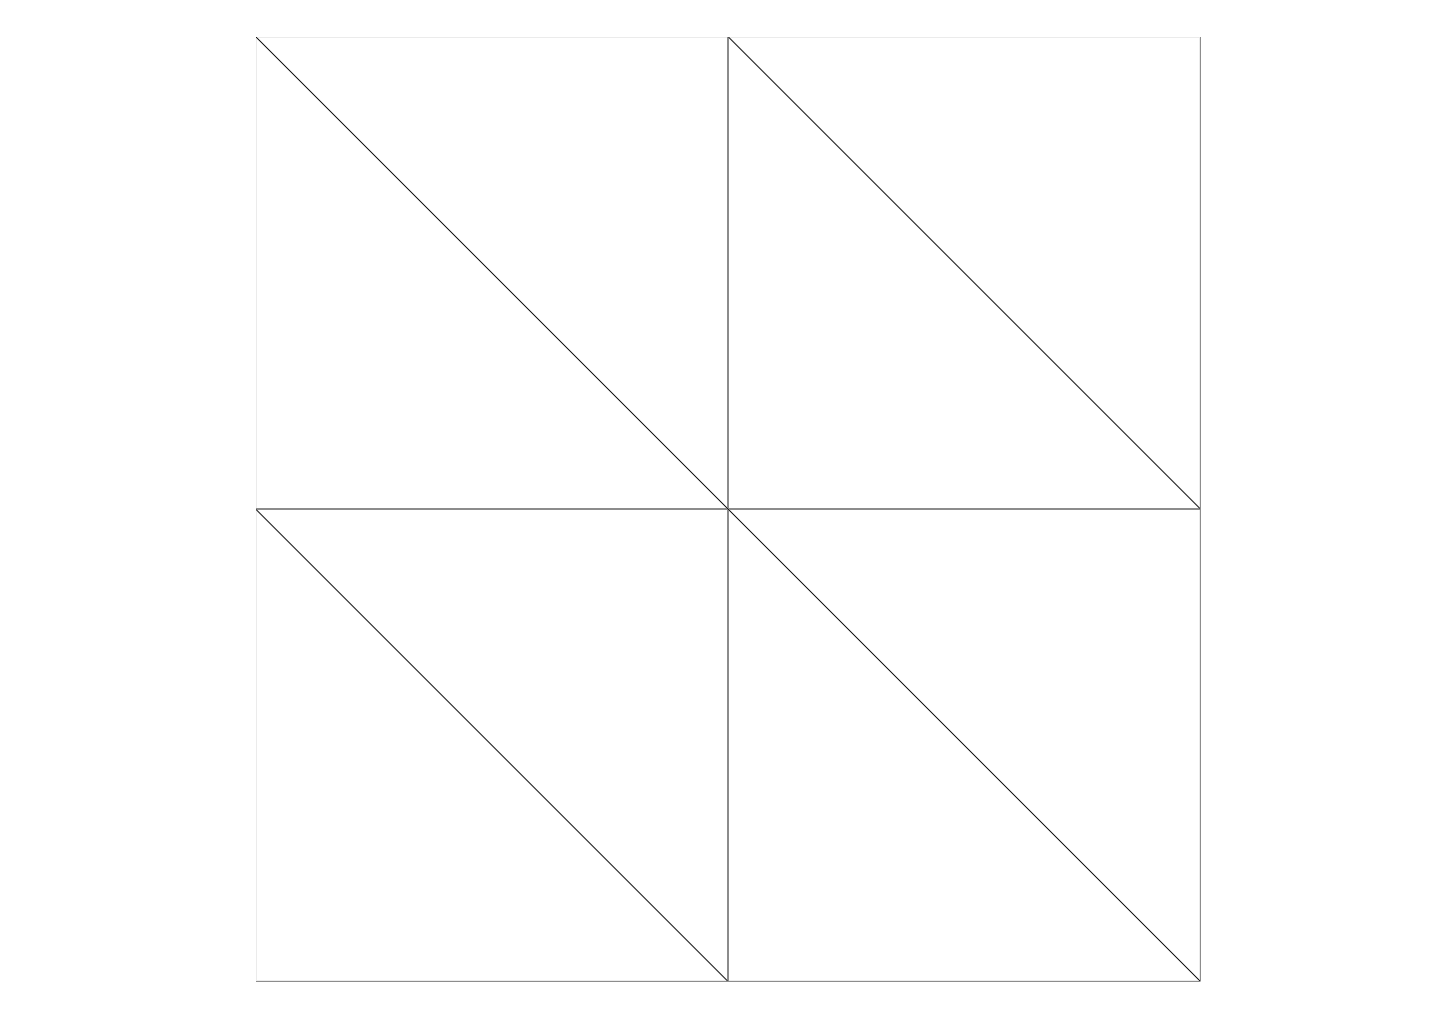
\includegraphics[width=\linewidth]
		{data/synthetic_meshes/square_tesselation_2tri_Dirac_delta_1_v9_f8_wireframe.png}
		\caption{$r=1$, wireframe}\label{fig:sq2.a}
	\end{subfigure}
	\begin{subfigure}[b]{0.32\linewidth}
		
\includegraphics[width=\linewidth]
		{data/synthetic_meshes/square_tesselation_2tri_Dirac_delta_1_v9_f8_funcvals_0iter_crop.png}
		\caption{$r=1$, $c=0$}\label{fig:sq2.b}
	\end{subfigure}
	\begin{subfigure}[b]{0.32\linewidth}
		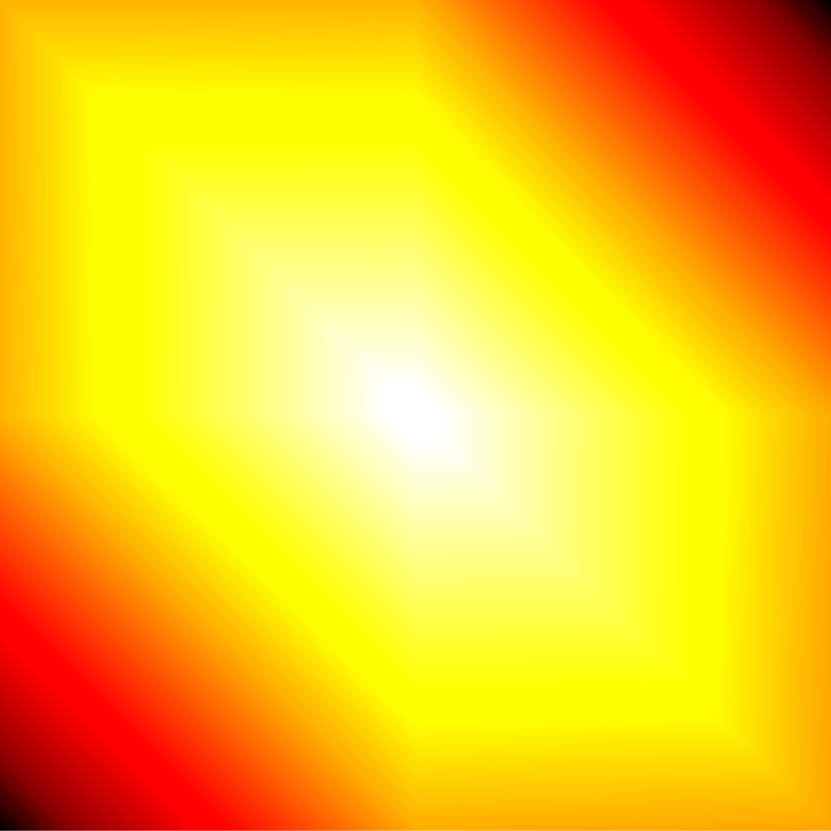
\includegraphics[width=\linewidth]
		{data/synthetic_meshes/square_tesselation_2tri_Dirac_delta_1_v9_f8_funcvals_1iter_crop.png}
		\caption{$r=1$, $c=1$}\label{fig:sq2.c}
	\end{subfigure}

	\bigskip
	\begin{subfigure}[b]{0.32\linewidth}
		
\includegraphics[width=\linewidth]
		{data/synthetic_meshes/square_tesselation_2tri_Dirac_delta_10_v441_f800_wireframe.png}
		\caption{$r=10$, wireframe}\label{fig:sq2.d}
	\end{subfigure}
	\begin{subfigure}[b]{0.32\linewidth}
		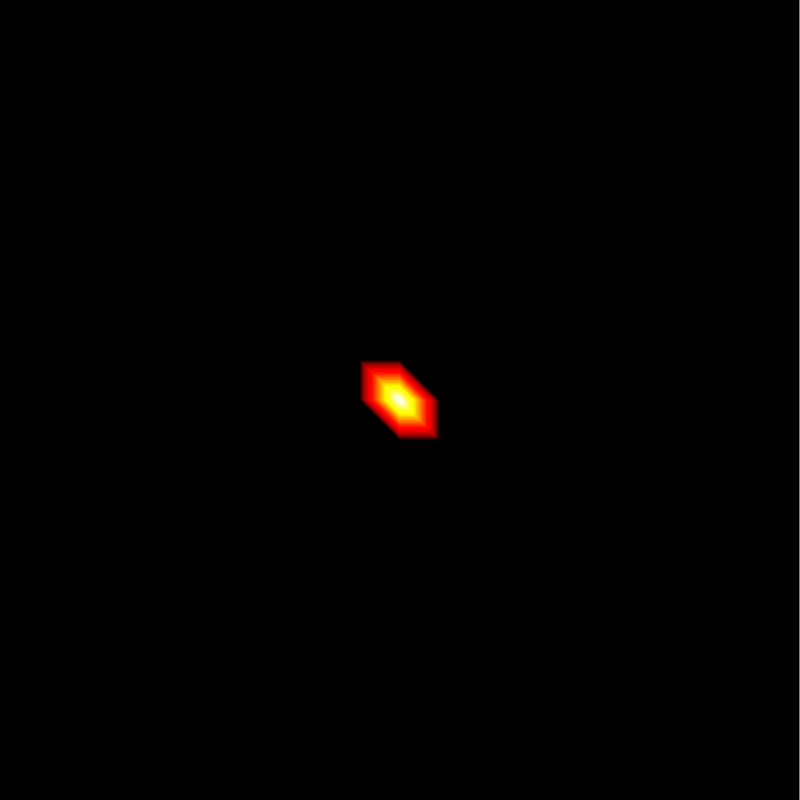
\includegraphics[width=\linewidth]
		{data/synthetic_meshes/square_tesselation_2tri_Dirac_delta_10_v441_f800_funcvals_0iter.png}
		\caption{$r=10$, $c=0$}\label{fig:sq2.e}
	\end{subfigure}
	\begin{subfigure}[b]{0.32\linewidth}
		
\includegraphics[width=\linewidth]
		{data/synthetic_meshes/square_tesselation_2tri_Dirac_delta_10_v441_f800_funcvals_100iter.png}
		\caption{$r=10$, $c=100$}\label{fig:sq2.f}
	\end{subfigure}
	\caption[Six views, comparing two differently sized of bisected square tessellations]{Comparison of two differently sized bisected square tessellations, generated with parameters $r$ set to 1 and 10: (a) $r=1$ in wireframe (b) $r=1$ colored by function value before convolving the filter (c) $r=1$ colored by function value after convolving the filter once (d) $r=10$ in wireframe (e) $r=10$ colored by function value before convoving the filter (f) $r=10$ colored by function value after convolving the filter 100 times.}
	\label{fig:sq2}
\end{figure}


%
%
%
%
\pagebreak
\subsection{Quadrisected Square Tessellations}
\label{ch6sSTDDssQST}
The synthetic mesh generator for quadirsected square tessellations generates meshes characterized by rings of squares around a center point, with the every corner made adjacent to the center point, quadrisecting each square into four equally sized isosceles, right triangles.

The smallest, non-trivial mesh, generated with the parameter $r$ equal to one, is composed of four squares around the center point, represented in total by only thirteen points and sixteen faces, however those numbers grow quickly with increasing parameter size $r$, according to the two equations
\begin{align}
	|\bP| &= 8r^2 + 4r + 1 \\
	|\bT| &= 16r^2
	\label{eq:sq4PointAndFaceCounts}
\end{align}

Figure~\ref{fig:sq2} shows a comparison of two differently sized quadrisected square tessellations, generated with parameters $r$ set to 1 and 10. Shown in (a) and (d) are each in wireframe, next in (b) and (e), each are colored by function value before convolving the filter, then in (c) $r=1$ is shown after convolving the filter once, and in (f) $r=10$ after convolving the filter 100 times. Notice the circular shape of the filter response in part (f).

\begin{figure}[ht]
	\begin{subfigure}[b]{0.32\linewidth}
		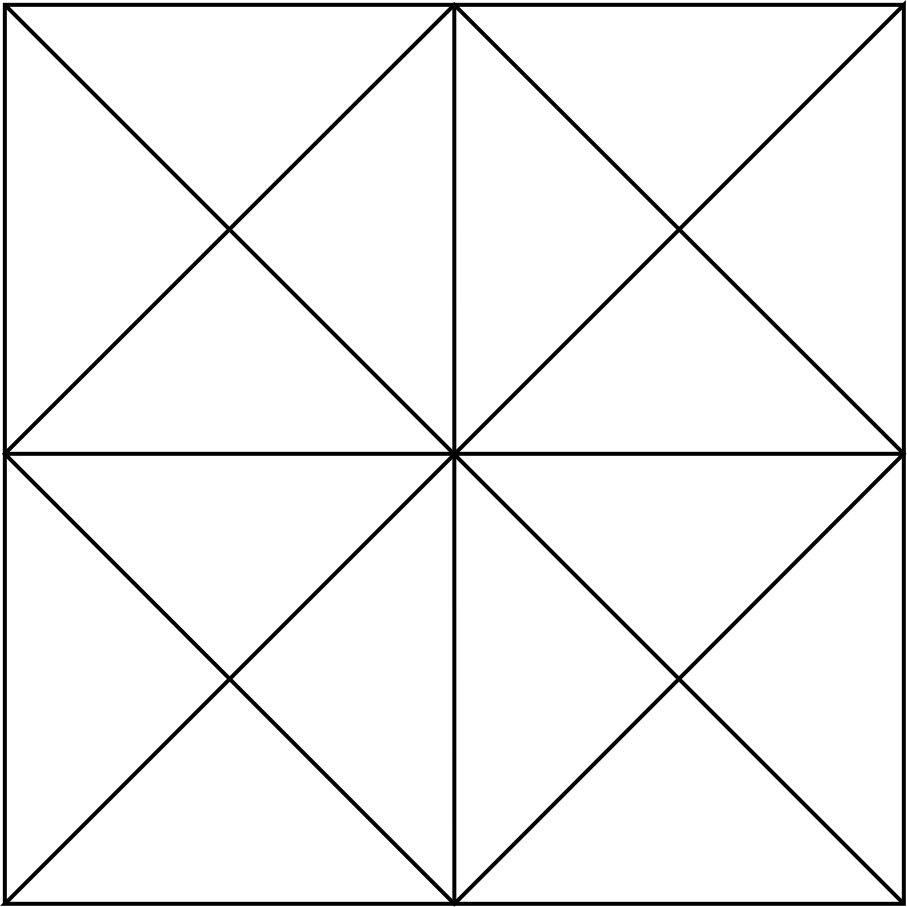
\includegraphics[width=\linewidth]
		{data/synthetic_meshes/square_tesselation_4tri_Dirac_delta_1_v13_f16_wireframe.png}
		\caption{$r=1$, wireframe}\label{fig:sq2.a}
	\end{subfigure}
	\begin{subfigure}[b]{0.32\linewidth}
		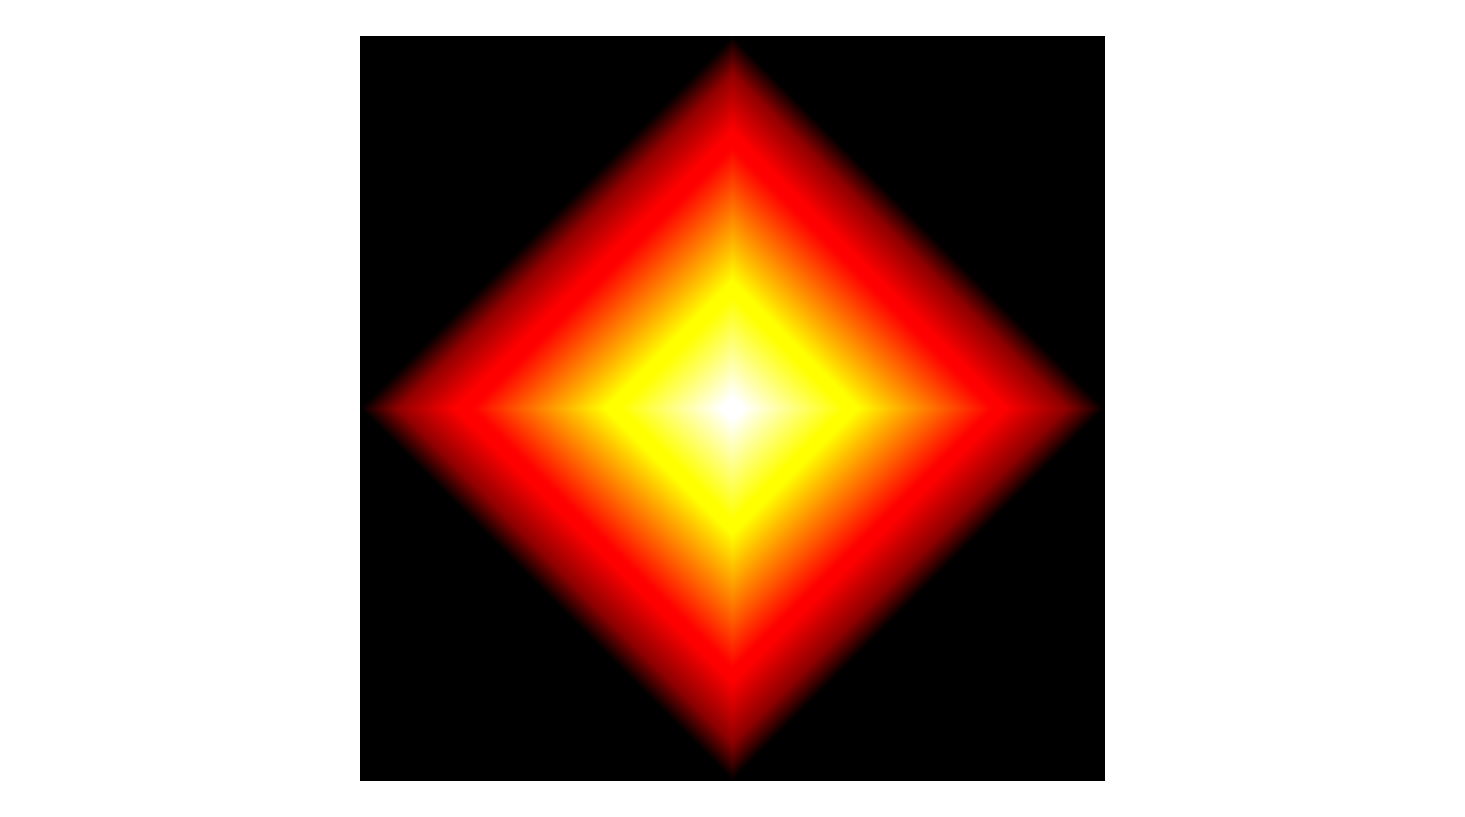
\includegraphics[width=\linewidth]
		{data/synthetic_meshes/square_tesselation_4tri_Dirac_delta_1_v13_f16_funcvals_0iter.png}
		\caption{$r=1$, $c=0$}\label{fig:sq2.b}
	\end{subfigure}
	\begin{subfigure}[b]{0.32\linewidth}
		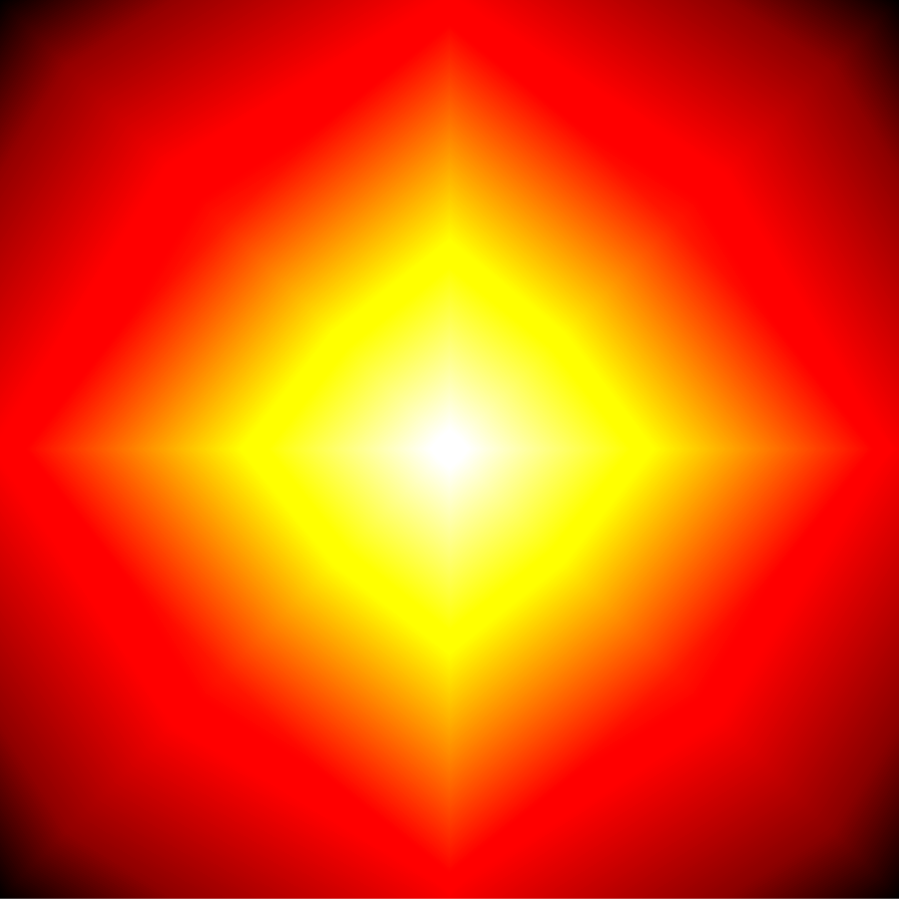
\includegraphics[width=\linewidth]
		{data/synthetic_meshes/square_tesselation_4tri_Dirac_delta_1_v13_f16_funcvals_1iter.png}
		\caption{$r=1$, $c=1$}\label{fig:sq2.c}
	\end{subfigure}

	\bigskip
	\begin{subfigure}[b]{0.32\linewidth}
		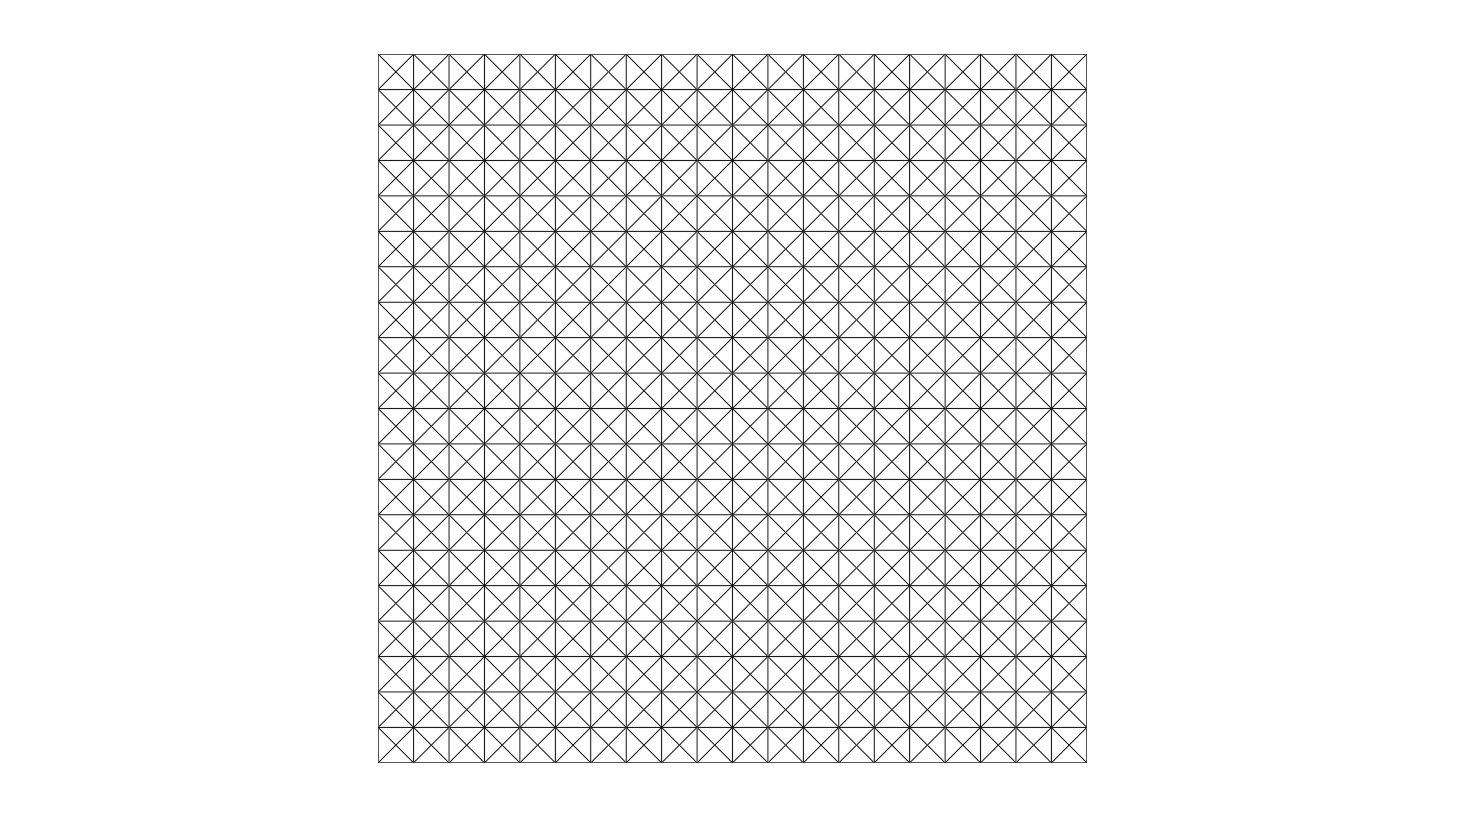
\includegraphics[width=\linewidth]
		{data/synthetic_meshes/square_tesselation_4tri_Dirac_delta_10_v841_f1600_wireframe.png}
		\caption{$r=10$, wireframe}\label{fig:sq2.d}
	\end{subfigure}
	\begin{subfigure}[b]{0.32\linewidth}
		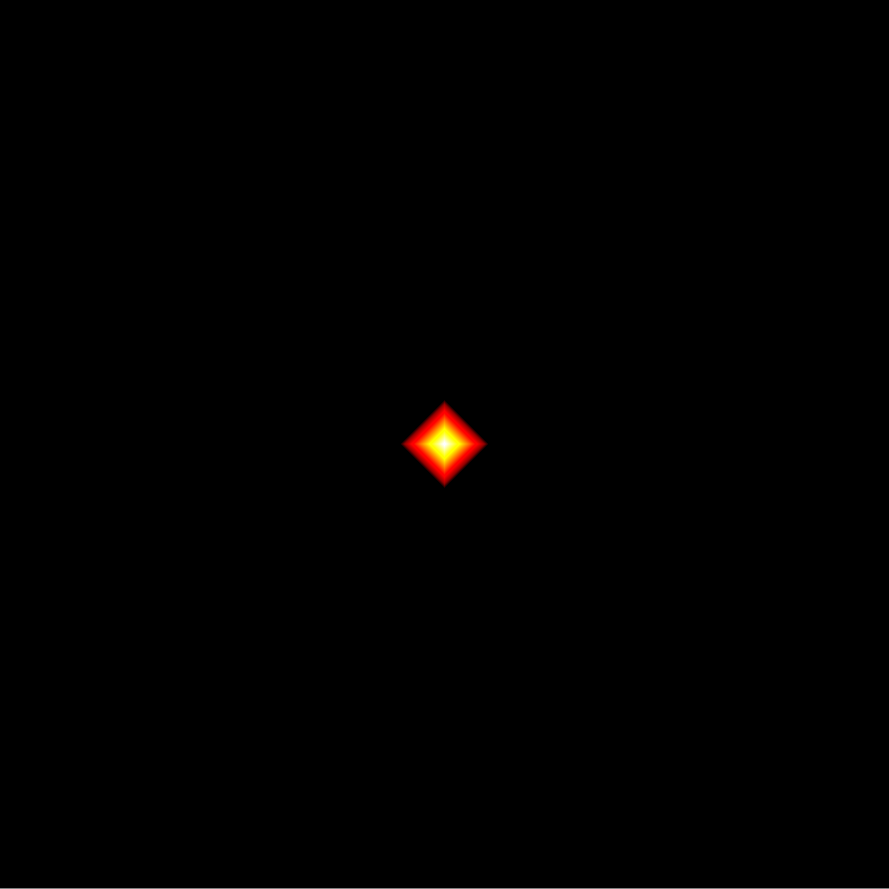
\includegraphics[width=\linewidth]
		{data/synthetic_meshes/square_tesselation_4tri_Dirac_delta_10_v841_f1600_funcvals_0iter.png}
		\caption{$r=10$, $c=0$}\label{fig:sq2.e}
	\end{subfigure}
	\begin{subfigure}[b]{0.32\linewidth}
		
\includegraphics[width=\linewidth]
		{data/synthetic_meshes/square_tesselation_4tri_Dirac_delta_10_v841_f1600_funcvals_100iter.png}
		\caption{$r=10$, $c=100$}\label{fig:sq2.f}
	\end{subfigure}
	\caption[Six views, comparing two differently sized of quadirsected square tessellations]{Comparison of two differently sized quadirsected square tessellations, generated with parameters $r$ set to 1 and 10: (a) $r=1$ in wireframe (b) $r=1$ colored by function value before convolving the filter (c) $r=1$ colored by function value after convolving the filter once (d) $r=10$ in wireframe (e) $r=10$ colored by function value before convoving the filter \newline(f) $r=10$ colored by function value after convolving the filter 100 times.}
	\label{fig:sq2}
\end{figure}


%
%
%
%
\pagebreak
\subsection{Hexagonal Tesselation}
\label{ch6sSTDDssHT}
The synthetic mesh generator for hexagonal tessellations generates meshes characterized by hexagons around one central hexagon, with each corner of the hexagons made adjacent to its own center point, creating six equilateral triangles per hexagon, and ensuring that every edge lengths in the mesh is of equal size.

The smallest, non-trivial mesh, generated with the parameter $r$ equal to zero, is composed of one hexagon around the center point, represented in total by only seven points and six faces, however those numbers grow quickly with increasing parameter size $r$, according to the two equations
\begin{align}
	|\bP| &= 3r^2 + 3r + 7 +\sum_{i=1}^r{6(2i + 1)}\\
	|\bT| &= 18r^2 + 18r + 6
	\label{eq:hexPointAndFaceCounts}
\end{align}

Figure~\ref{fig:sq2} shows a comparison of two differently sized hexagonal tessellations, generated with parameters $r$ set to 1 and 10. Shown in (a) and (d) are each in wireframe, next in (b) and (e), each are colored by function value before convolving the filter, then in (c) $r=1$ is shown after convolving the filter twice, and in (f) $r=10$ after convolving the filter 200 times.

\begin{figure}[ht]
	\begin{subfigure}[b]{0.32\linewidth}
		
\includegraphics[width=\linewidth]
		{data/synthetic_meshes/hexagonal_tessellation_Dirac_delta_1_v31_f42_wireframe.png}
		\caption{$r=1$, wireframe}\label{fig:hex.a}
	\end{subfigure}
	\begin{subfigure}[b]{0.32\linewidth}
		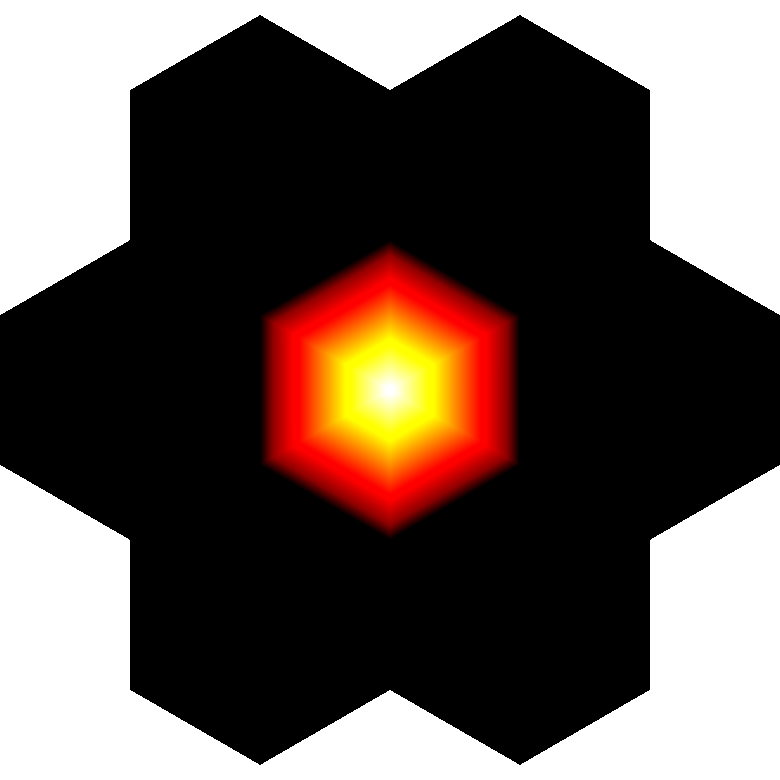
\includegraphics[width=\linewidth]
		{data/synthetic_meshes/hexagonal_tessellation_Dirac_delta_1_v31_f42_funcvals_0iter_crop.png}
		\caption{$r=1$, $c=0$}\label{fig:hex.b}
	\end{subfigure}
	\begin{subfigure}[b]{0.32\linewidth}
		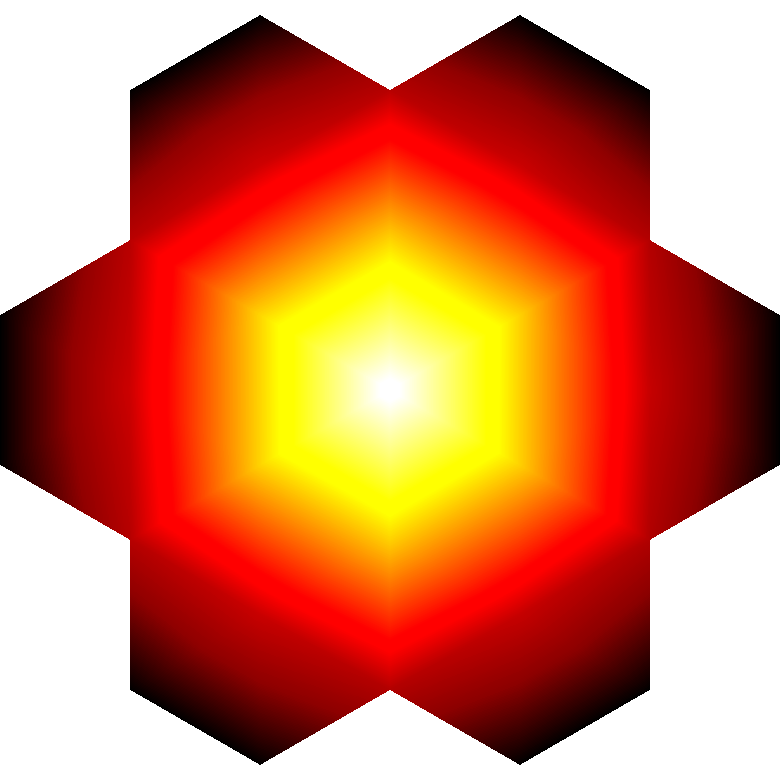
\includegraphics[width=\linewidth]
		{data/synthetic_meshes/hexagonal_tessellation_Dirac_delta_1_v31_f42_funcvals_2iter_crop.png}
		\caption{$r=1$, $c=2$}\label{fig:hex.c}
	\end{subfigure}

	\begin{subfigure}[b]{0.32\linewidth}
		
\includegraphics[width=\linewidth]
		{data/synthetic_meshes/hexagonal_tessellation_Dirac_delta_10_v1057_f1986_wireframe.png}
		\caption{$r=10$, wireframe}\label{fig:hex.d}
	\end{subfigure}
	\begin{subfigure}[b]{0.32\linewidth}
		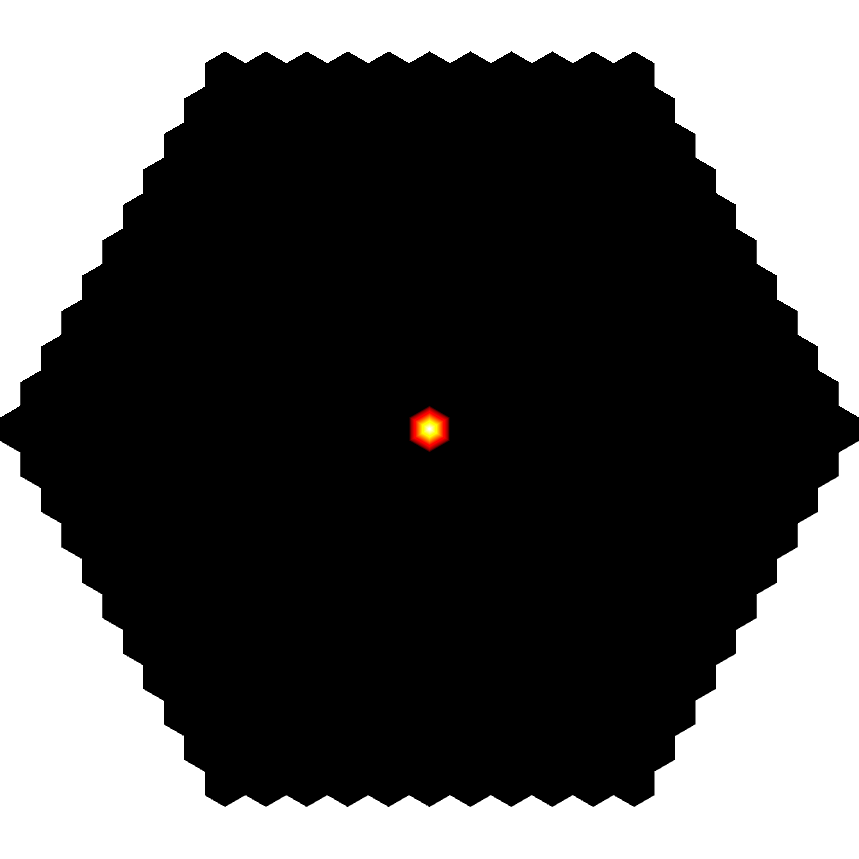
\includegraphics[width=\linewidth]
		{data/synthetic_meshes/hexagonal_tessellation_Dirac_delta_10_v1057_f1986_funcvals_0iter_crop.png}
		\caption{$r=10$, $c=0$}\label{fig:hex.e}
	\end{subfigure}
	\begin{subfigure}[b]{0.32\linewidth}
		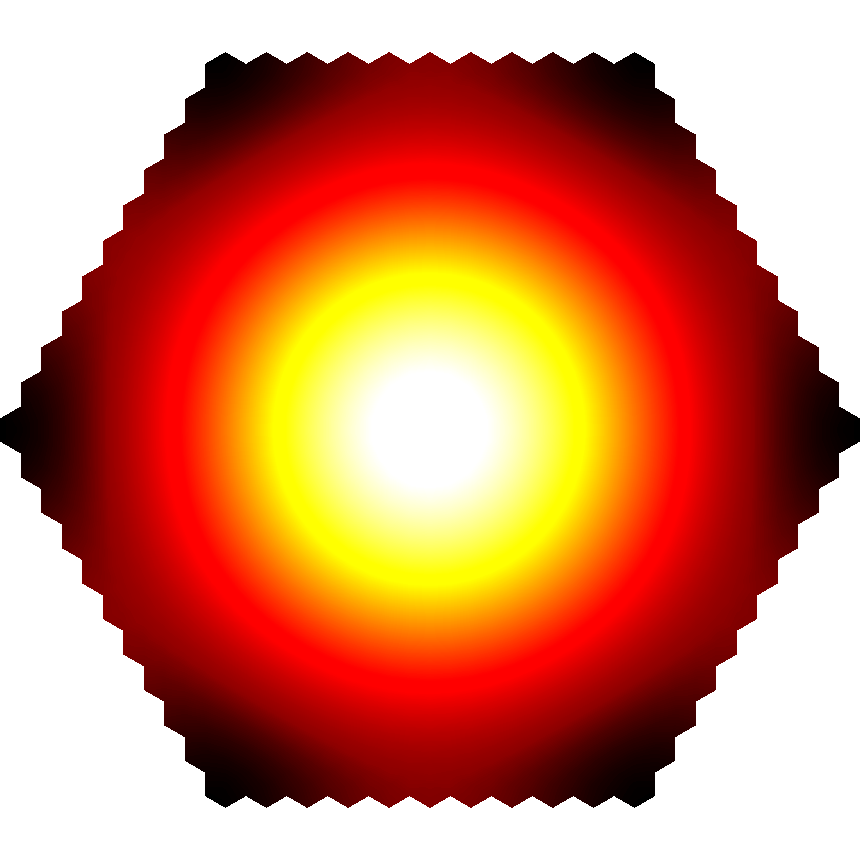
\includegraphics[width=\linewidth]
		{data/synthetic_meshes/hexagonal_tessellation_Dirac_delta_10_v1057_f1986_funcvals_200iter_crop.png}
		\caption{$r=10$, $c=200$}\label{fig:hex.f}
	\end{subfigure}
	\caption[Six Views Comparing Hexagonal Tessellations]{Comparison of two differently-sized, hexagonal tessellations, generated with parameters $r$ set to 1 and 10. (a) $r=1$ in wireframe, (b) $r=1$ colored by function value before convolving the filter, (c) $r=1$ colored by function value after convolving the filter once, (d) $r=10$ in wireframe, (e) $r=10$ colored by function value before convoving the filter, and (f) $r=10$ colored by function value after convolving the filter 200 times.}
	\label{fig:hex}
\end{figure}


%
%
%
%
\pagebreak
\subsection{Random Triangulated Discs}
\label{ch6sSTDDssRTD}
The synthetic mesh generator for random triangulated discs generates meshes characterized by radially bounded, uniformly distributed, random points,  triangulated following the well-studied method originally presented by of Delaunay~\cite{Delaunay34}. Generating random triangulated discs requires two parameters, the radius of the disc $r$, and the number of points $p$. The parameters were chosen to ensure parity with the sizes and point density of the other synthetic meshes, as summarized in Table~\ref{tbl:rdisc}.
\vspace*{-.5\baselineskip}
\begin{table}[ht]
\begin{tabular}{rrr|rrr}
\textbf{Radius $r$} & \textbf{Points $p$} & \textbf{Faces} & \textbf{Radius $r$} & \textbf{Points $p$} & \textbf{Faces}\\
\hline
    1 &         11 &          12 &   100 &     60,401 &     120,668\\
    3 &         67 &         119 &   300 &    541,201 &   1,082,132\\
   10 &        641 &       1,252 & 1,000 &  6,004,001 &  12,007,382\\
   30 &      5,521 &      10,971 & 3,000 & 54,012,001 & 108,022,714%
\caption{Summary of the parameters used with the random triangulated disc generator\label{tbl:rdisc}}
\end{tabular}
\end{table}

Figure~\ref{fig:sq2} shows a comparison of two differently sized, random triangulated discs, generated with parameters $r$ set to 1 and 10, and parameters $p$ set to 11 and 641. Shown in (a) and (d) are each in wireframe, next in (b) and (e), each are colored by function value before convolving the filter, then in (c) $r=1$ is shown after convolving the filter twice, and in (f) $r=10$ after convolving the filter 10,000 times.

\vspace*{-\baselineskip}
\begin{figure}[ht]
	\begin{subfigure}[b]{0.32\linewidth}
		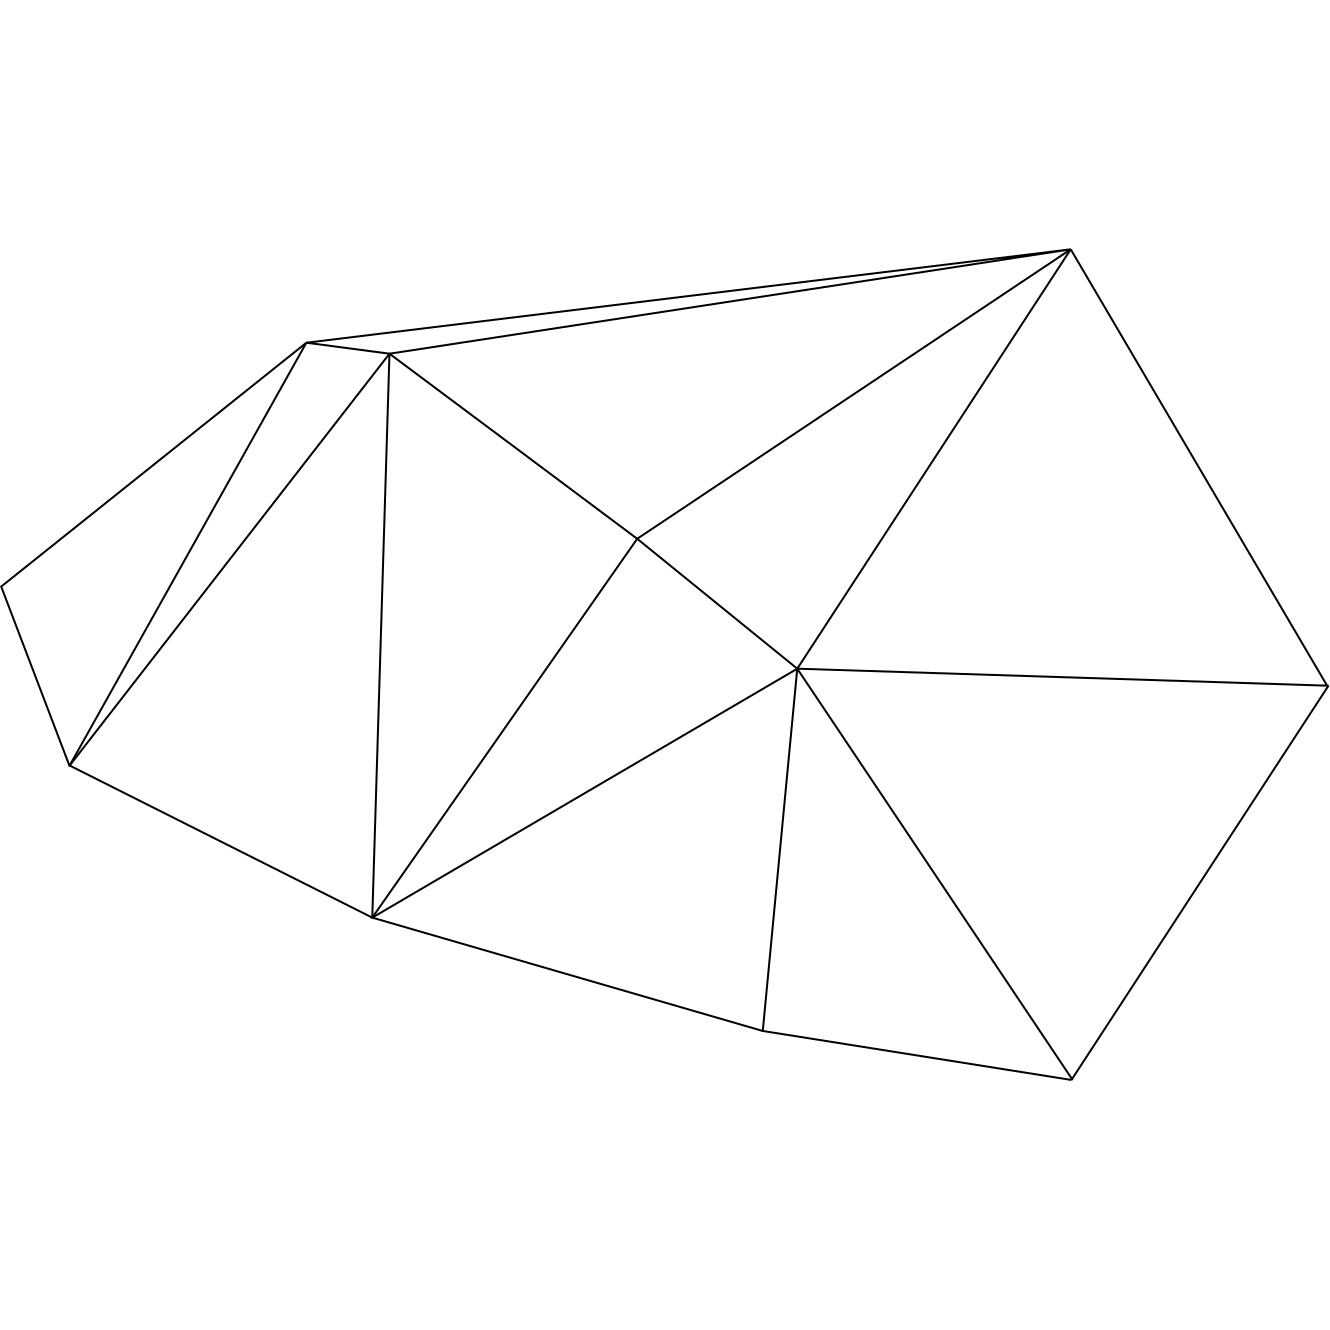
\includegraphics[width=\linewidth]
		{data/synthetic_meshes/random_circle_tessellation_Dirac_delta_1_v11_f12_wireframe.png}
		\caption{$r=1$, $p=11$, wireframe}\label{fig:rcirc.a}
	\end{subfigure}
	\begin{subfigure}[b]{0.32\linewidth}
		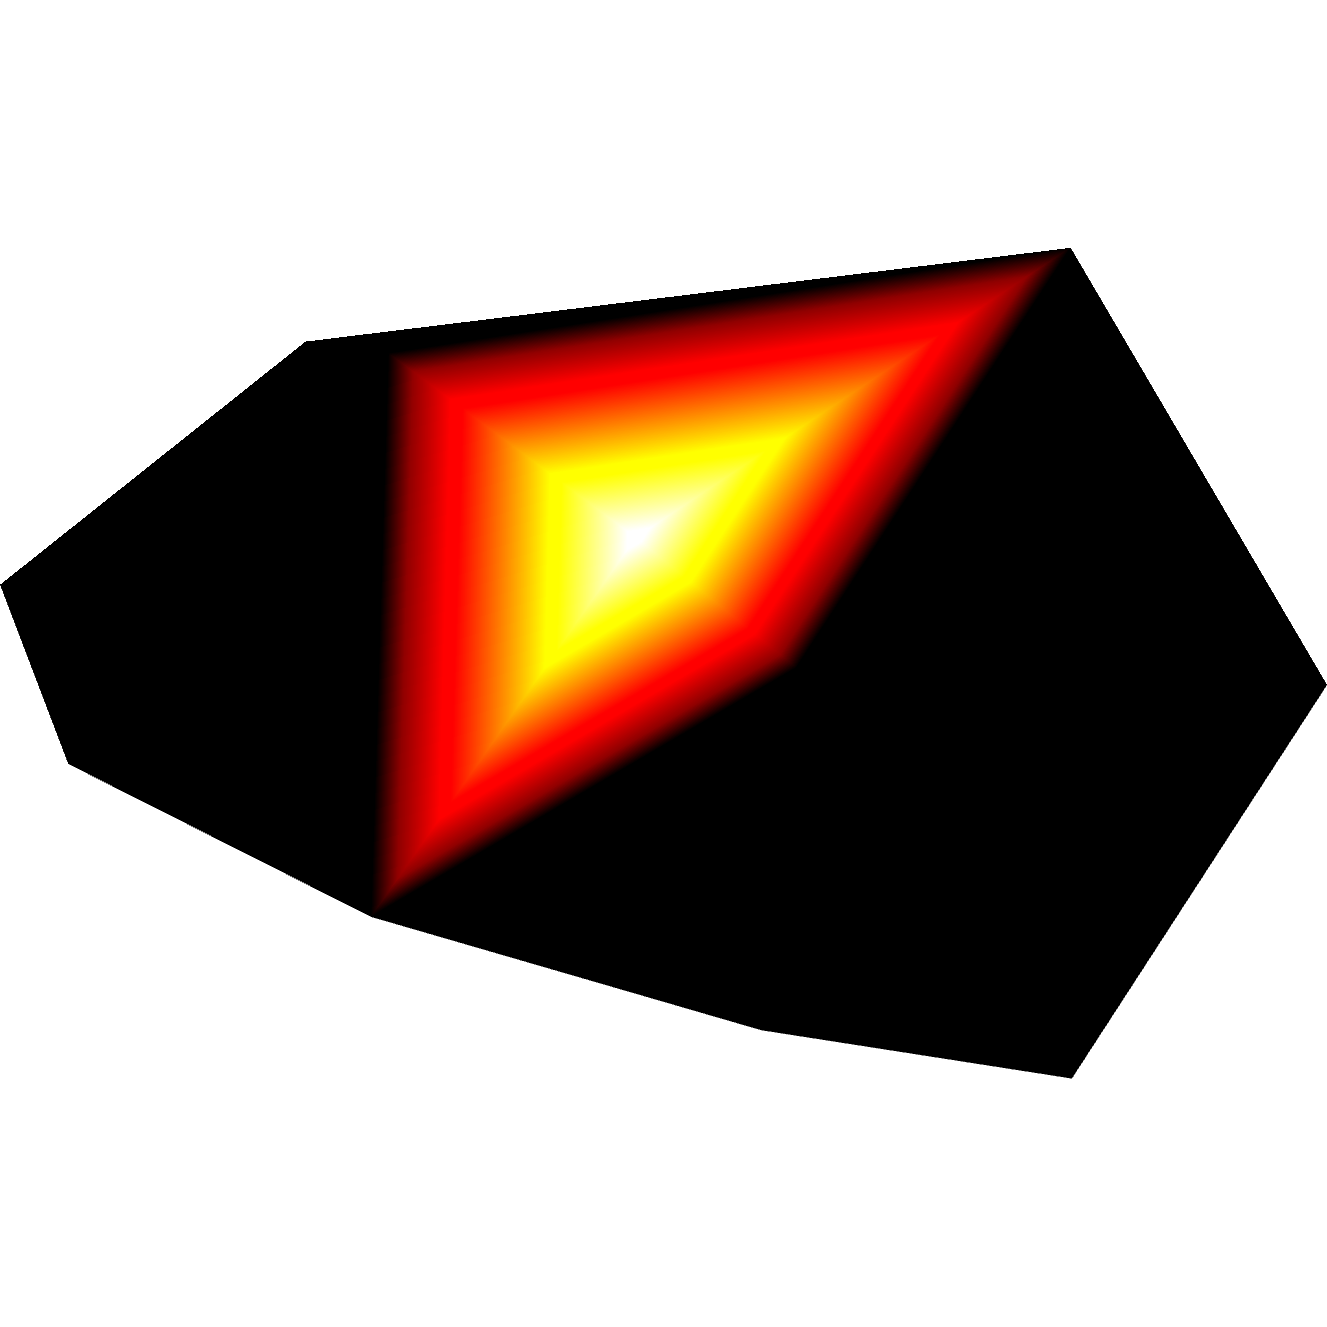
\includegraphics[width=\linewidth]
		{data/synthetic_meshes/random_circle_tessellation_Dirac_delta_1_v11_f12_funcvals_0iter.png}
		\caption{$r=1$, $p=11$, $c=0$}\label{fig:rcirc.c}
	\end{subfigure}
	\begin{subfigure}[b]{0.32\linewidth}
		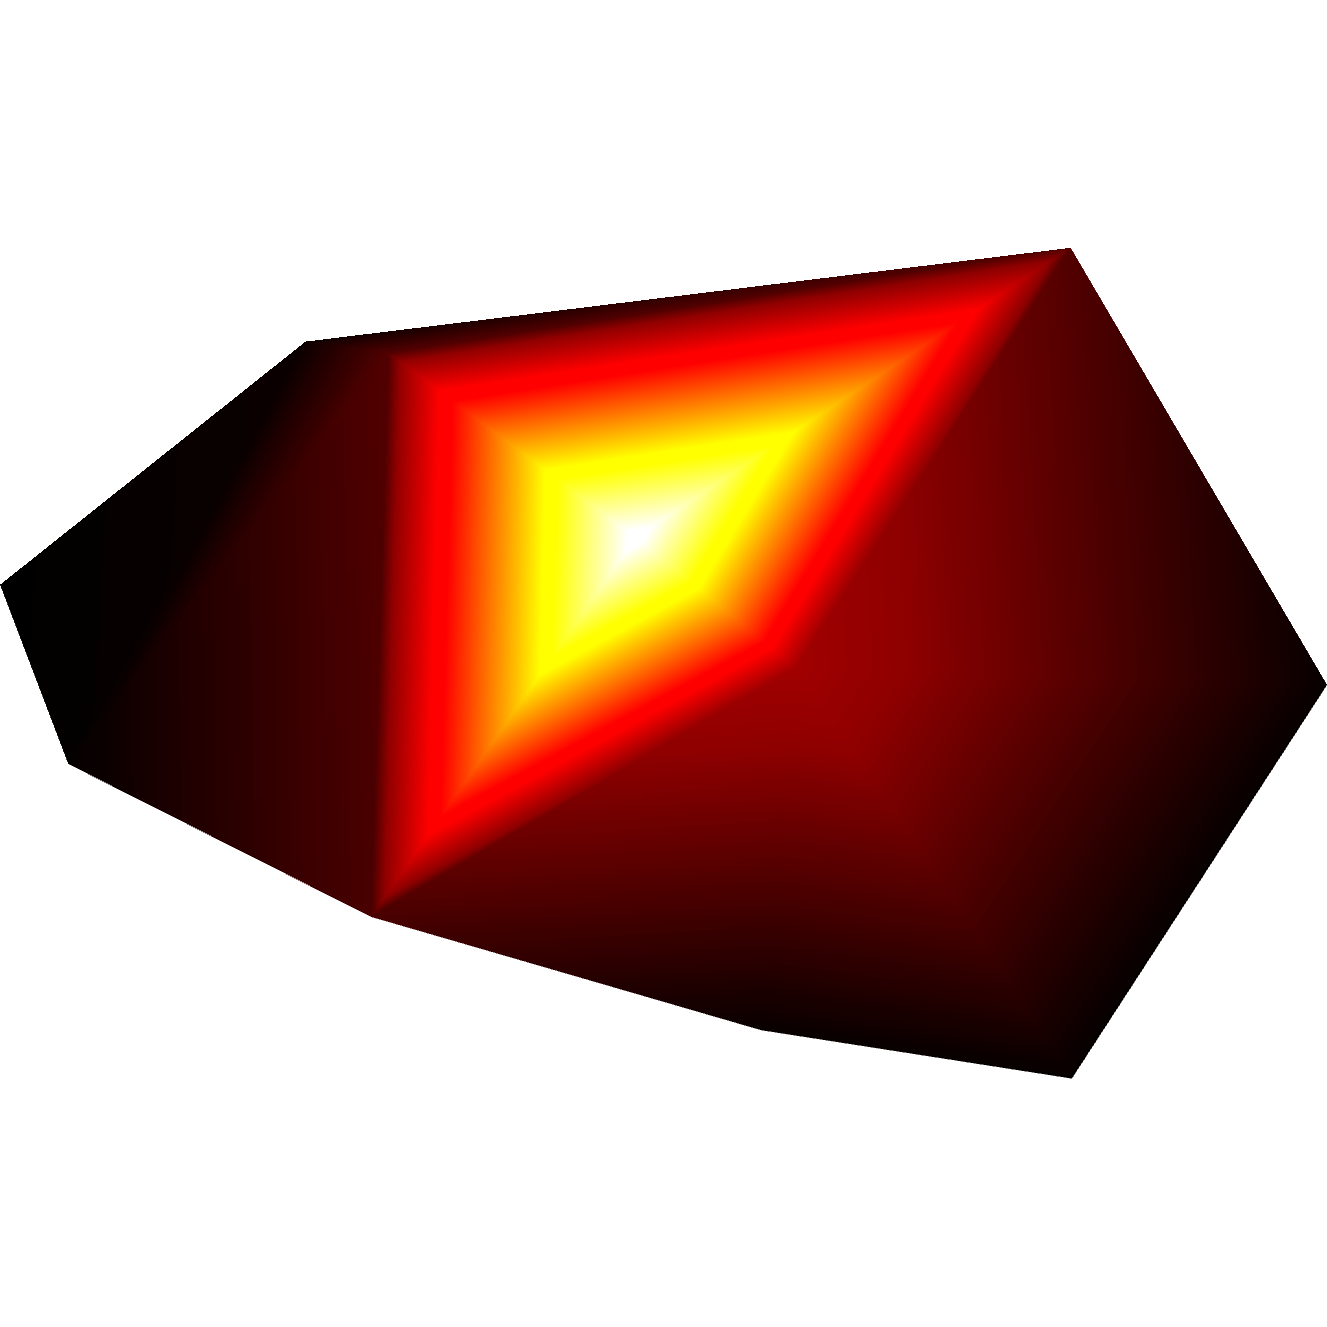
\includegraphics[width=\linewidth,]
		{data/synthetic_meshes/random_circle_tessellation_Dirac_delta_1_v11_f12_funcvals_2iter.png}
		\caption{$r=1$, $p=11$, $c=2$}\label{fig:rcirc.e}
	\end{subfigure}

	\bigskip
	\begin{subfigure}[b]{0.32\linewidth}
		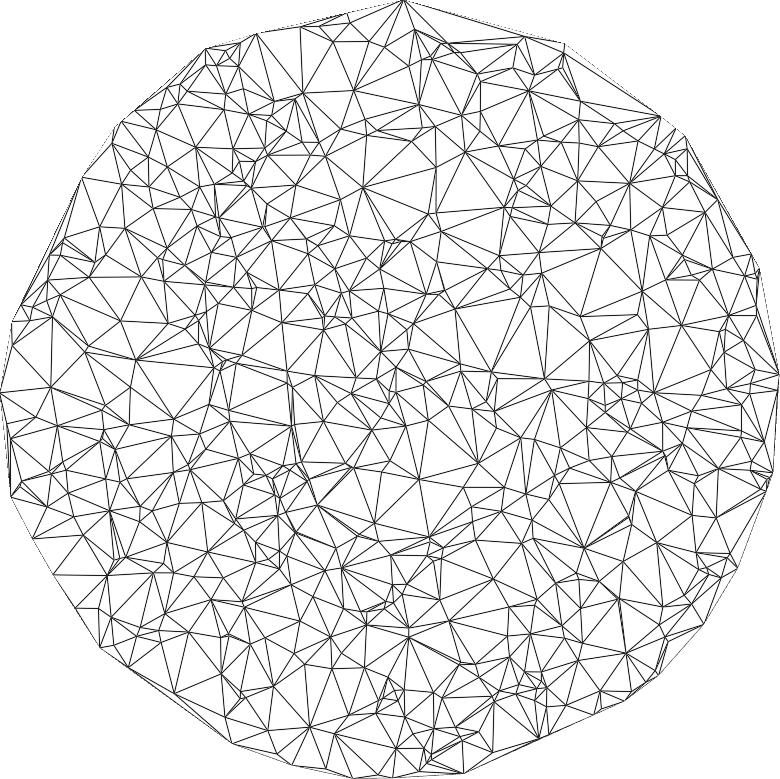
\includegraphics[width=\linewidth]
		{data/synthetic_meshes/random_circle_tessellation_Dirac_delta_10_v641_f1252_wireframe.png}
		\caption{$r=10$, $p=641$, wireframe}\label{fig:rcirc.b}
	\end{subfigure}
	\begin{subfigure}[b]{0.32\linewidth}
		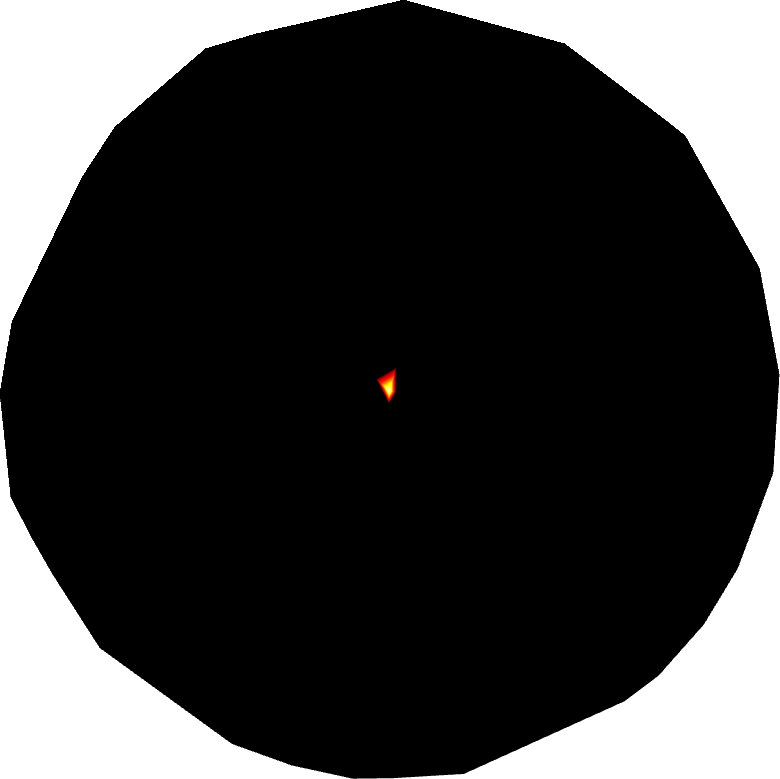
\includegraphics[width=\linewidth]
		{data/synthetic_meshes/random_circle_tessellation_Dirac_delta_10_v641_f1252_funcvals_0iter.png}
		\caption{$r=10$, $p=641$, $c=0$}\label{fig:rcirc.d}
	\end{subfigure}
	\begin{subfigure}[b]{0.32\linewidth}
		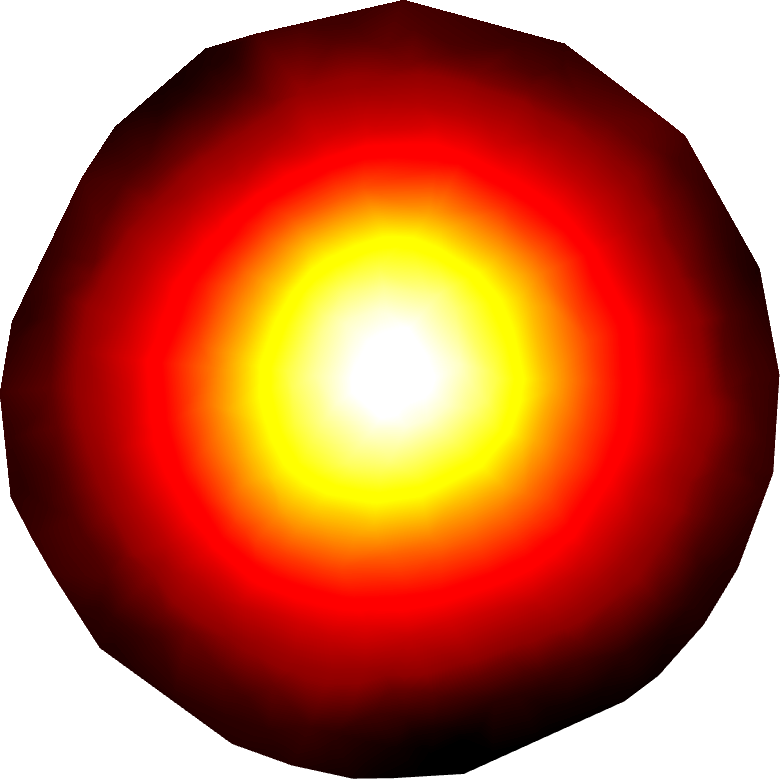
\includegraphics[width=\linewidth]
		{data/synthetic_meshes/random_circle_tessellation_Dirac_delta_10_v641_f1252_funcvals_10000iter.png}
		\caption{$r=10$, $p=641$, $c=10^4$}\label{fig:rcirc.f}
	\end{subfigure}
	\caption[Six views, comparing two differently sized, random triangulated discs]{Comparison of two differently sized, random triangulated discs, generated with parameters $r$ set to 1 and 10, and parameters $p$ set to 11 and 641: (a) $r=1$, $p=11$ in wireframe (b) $r=1$, $p=11$ colored by function value before convolving the filter (c) $r=1$, $p=11$ colored by function value after convolving the filter twice (d) $r=10$, $p=641$ in wireframe (e) $r=10$, $p=641$ colored by function value before convoving the filter (f) $r=10$, $p=641$ colored by function value after convolving the filter 10,000 times.}
	\label{fig:rdisc}
\end{figure}



%
%
%
%
%
%
\pagebreak
\section{Acquired \tdd{}}
\label{ch6sATDD}
Each of the three acquired \tdd{} examples used in our experiments, the partial model of the University of Heidelberg seal, the flat surface from ILATO, and the Stanford Bunny, were initially processed with the GigaMesh framework in order to generate a scalar field of function values using the Multi-Scale Integral Invariants filter, MSII~\cite{Mara12}. Also, we experience two kinds of difficulties, error propagation and diminishing effectiveness when convolving the filter, highlighting the complexity of working with acquired \tdd{}.

%
%
%
%
\subsection{The University of Heidelberg Seal}
\label{ch6sATDDssUHS}
This acquired \tdd{} is a partial model, comprised of 397,210 points and 789,406 faces, taken from the center of a 3D-scan of the seal of the University of Heidelberg, as established in 1386, and stored by the Univeristy of Heidelberg Archives. The original data was captured with a high resolution 3D-scanner and is stored in the heiDATA dataverse of the IWR Computer Graphics~\cite{Unisiegel}.

Figure~\ref{fig:unisiegel} shows three views of the partial model taken from the University of Heidelberg seal: in wireframe, colored by function values generated by applying the MSII filter, before convolving \fors{t}, and colored by function value after convolving \fors{t} 100 times.

\begin{figure}[ht]
	\begin{subfigure}[b]{0.32\linewidth}
		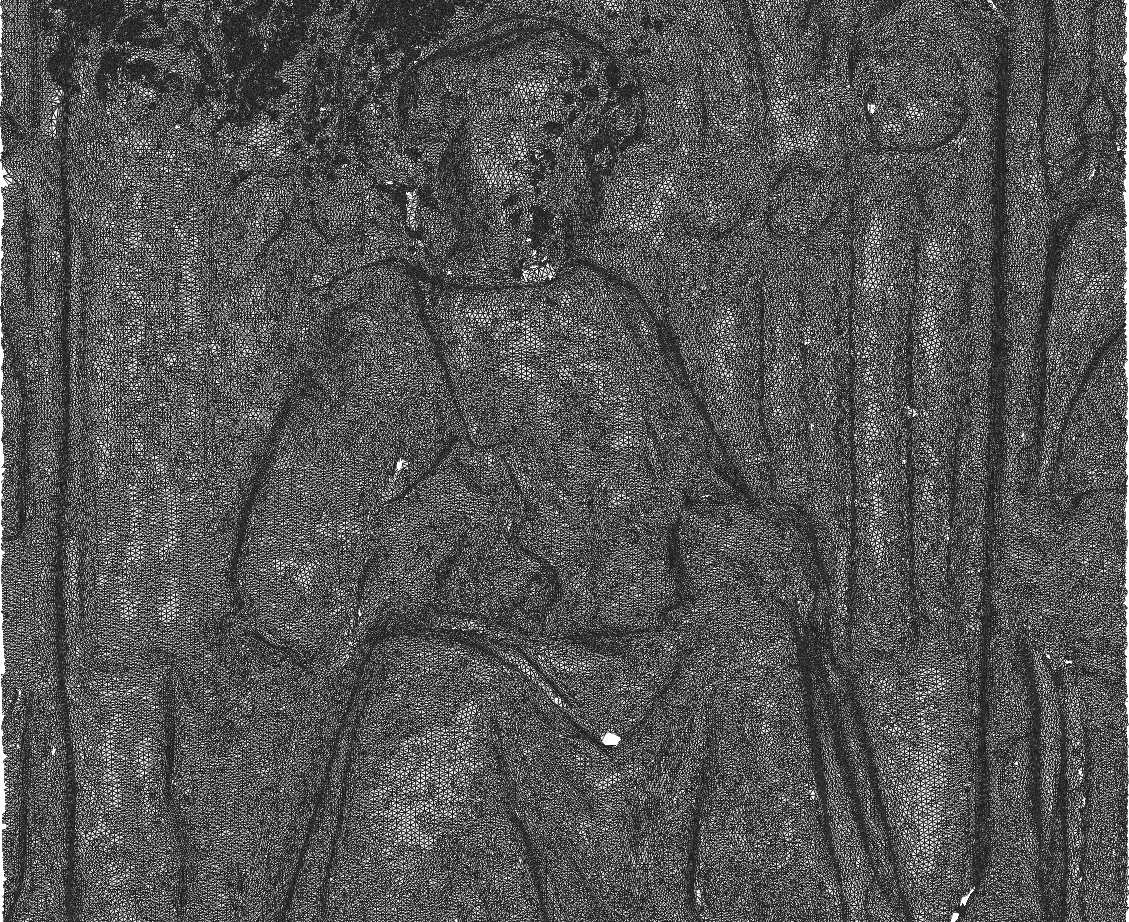
\includegraphics[width=\linewidth]{data/acquired_meshes/unisiegel_wireframe.png}
		\caption{wireframe}\label{fig:unisiegel.a}
	\end{subfigure}
	\begin{subfigure}[b]{0.32\linewidth}
		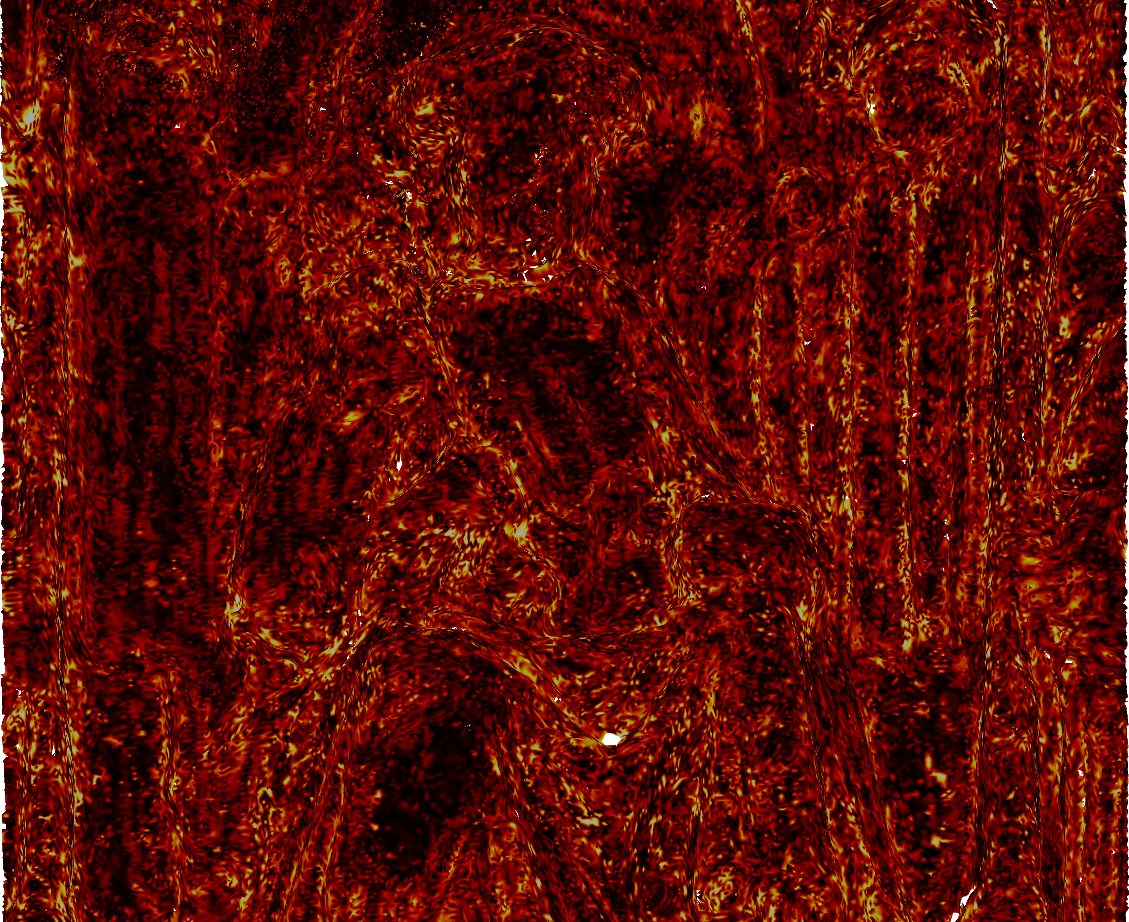
\includegraphics[width=\linewidth]{data/acquired_meshes/unisiegel_0iter.png}
		\caption{$c=0$}\label{fig:unisiegel.b}
	\end{subfigure}
	\begin{subfigure}[b]{0.32\linewidth}
		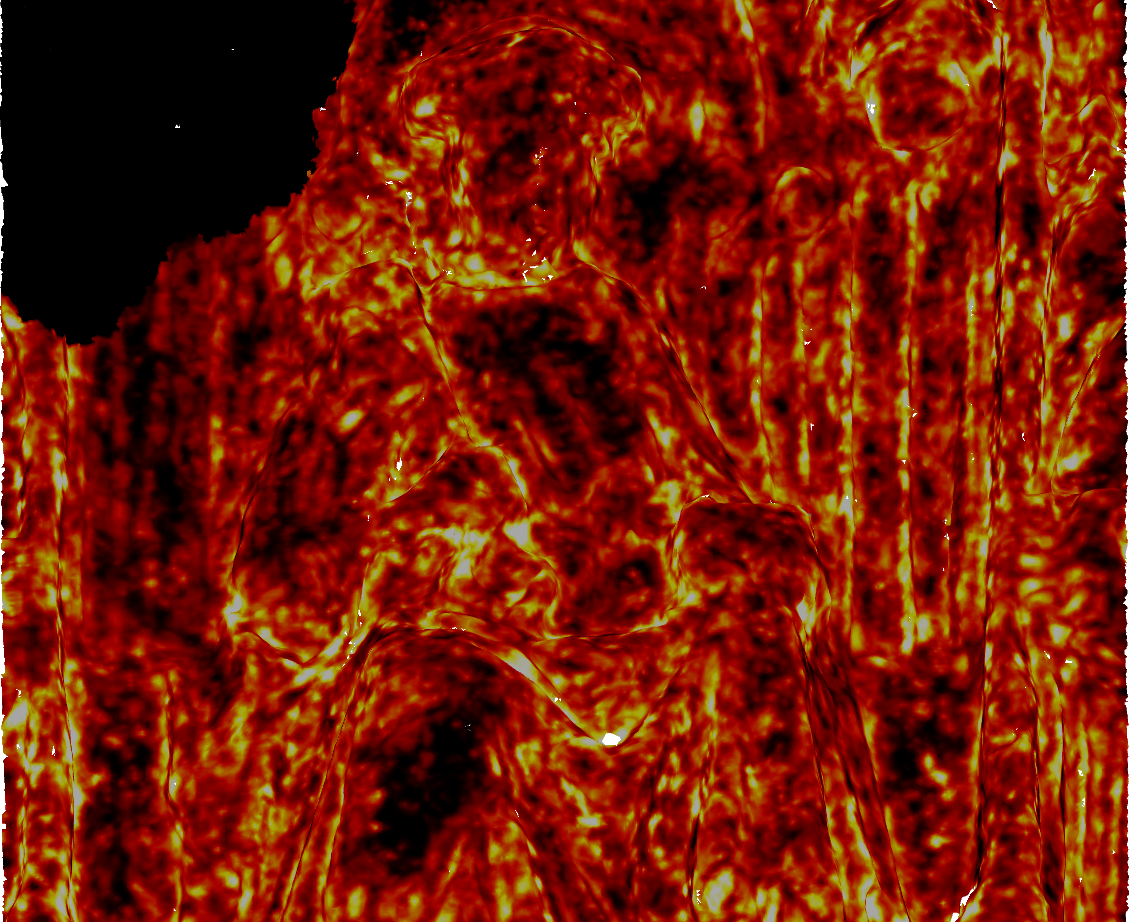
\includegraphics[width=\linewidth]{data/acquired_meshes/unisiegel_100iter.png}
		\caption{$c=100$}\label{fig:unisiegel.c}
	\end{subfigure}
	\caption[Three views of the Univeristy of Heidelberg Seal]{Three views of the Univeristy of Heidelberg seal (a) in wireframe, (b) colored by \gls{tMSIIf} value before convolving the filter, (c) colored by function value after convolving the filter 100 times.}
	\label{fig:unisiegel}
\end{figure}


There exist several holes in this \tdd{}, including the relatively large hole in the lap of the figure, just below the center of each image. However, as \fors{t} convolves over every point, considering each neighborhood in isolation, the convexity of the entire mesh is inconsequential, and faces adjacent to holes are treated the same as faces adjacent to borders, where \wmfv{s} are averaged over the sectors of the geodesic disc which do exist.

Also notice the large black area in the top left corner of (c). Due to one of the many non-manifold, irregularities of the original mesh, an error occurred when the filter attempted to divide a function value by zero-sized area, and that error then propagated to every adjacent neighborhood in every subsequent iteration. Using the ``Automatic Mesh Polishing'' feature in GigaMesh~\cite[p.~29-32]{Mara12}~\cite[p.7]{Giga17} before convolving the filter, completely eliminates the problem, however further modifications to \fors{t} algorithm may be necessary to ensure the overall stability of the filter.

%
%
%
%
\subsection{A flat surface from \gls{ILATO}}
\label{ch6sATDDssI}
This acquired \tdd{} is a partial model, comprised of 56,215 points and 111,311 faces, taken from the center of sample 1A of the set of industrial samples presented by the \gls{ILATO} project~, Improving Limited Angle computed Tomography by Optical data integration\cite{ILATO14}. The original data was obtained by scanning an aluminum block with brushed surface finish, with a Breuckmann scanners SmartScan 3D~\cite{Bayer16}.

Figure~\ref{fig:ILATO} shows four views of the partial model taken from \gls{ILATO} sample 1a: in wireframe, colored by function values generated by applying the MSII filter, before convolving \fors{t}, colored by function value after convolving \fors{t} 1000 times, and then again after convolving the filter 3000 times.
\begin{figure}[ht]
	\begin{subfigure}[b]{0.49\linewidth}
		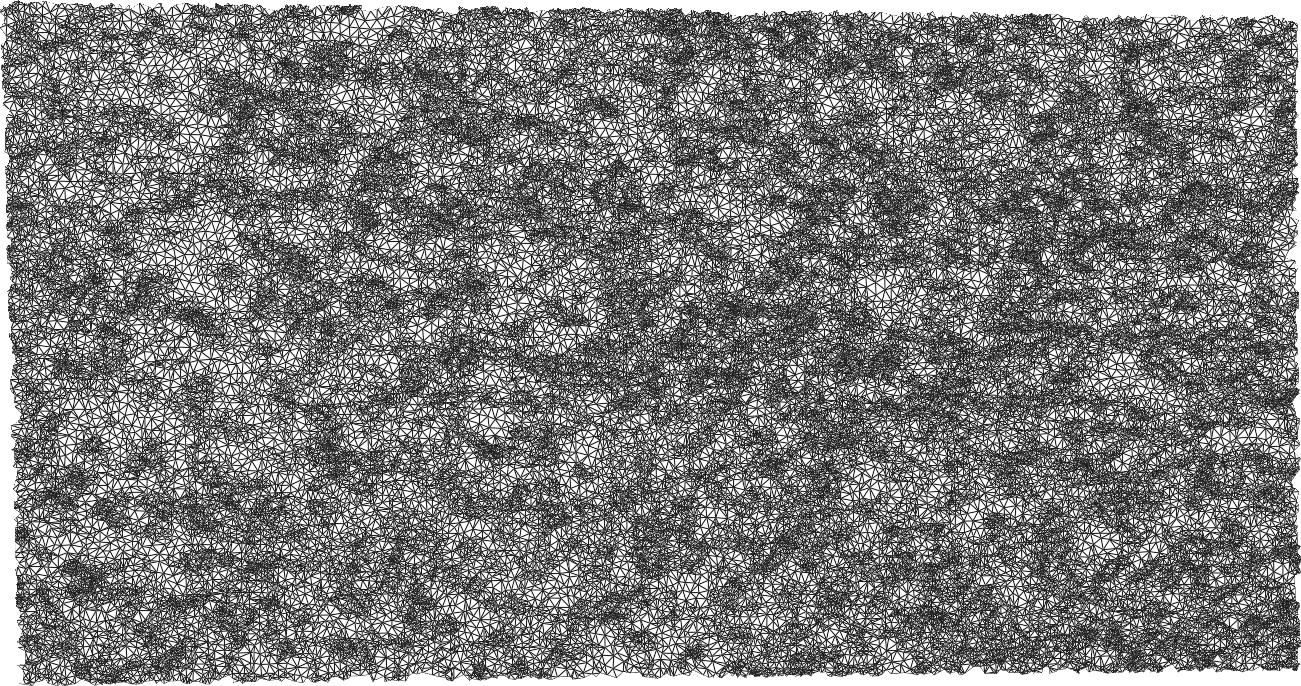
\includegraphics[width=\linewidth]
		{data/acquired_meshes/ILATO_1A_SM2066-HE5-60_070214_merged_GMO_r1_n4_v256_wireframe.png}
		\caption{wireframe}\label{ILATO:bun.a}
	\end{subfigure}
	\begin{subfigure}[b]{0.49\linewidth}
		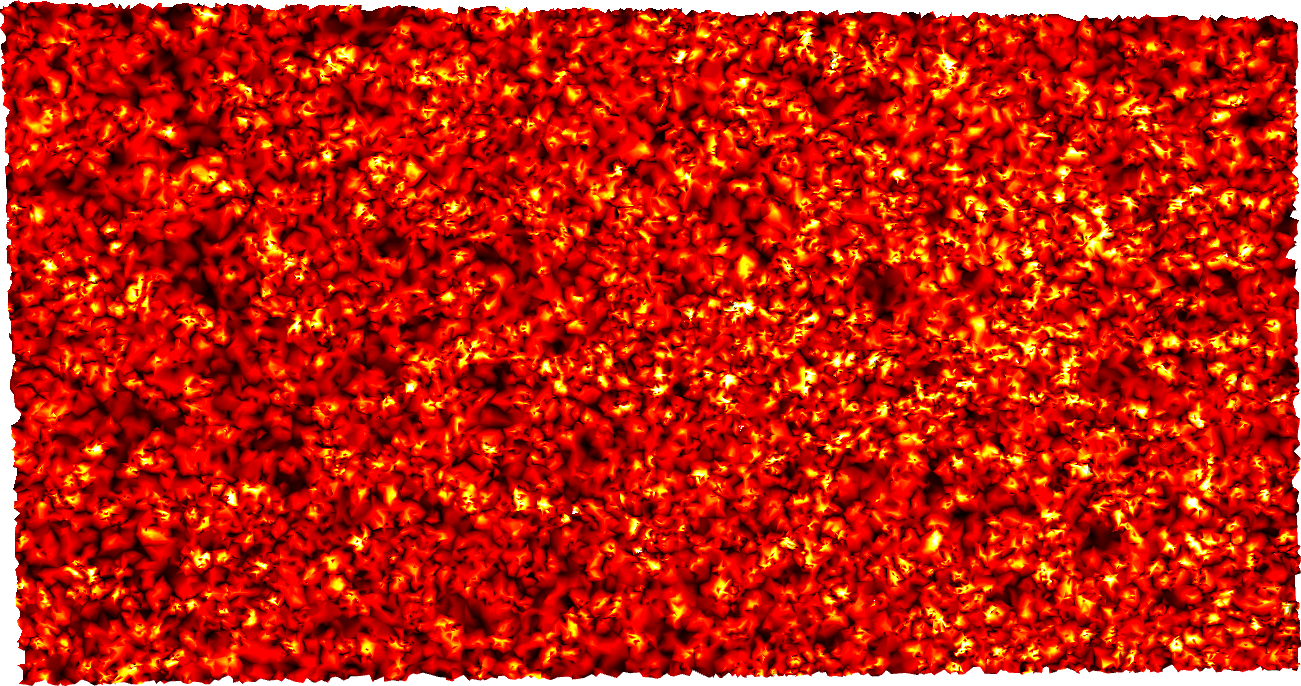
\includegraphics[width=\linewidth]
		{data/acquired_meshes/ILATO_1A_SM2066-HE5-60_070214_merged_GMO_r1_n4_v256_funcvals_0iter.png}
		\caption{$c=0$}\label{fig:buILATOn.b}
	\end{subfigure}

	\bigskip
	\begin{subfigure}[b]{0.49\linewidth}
		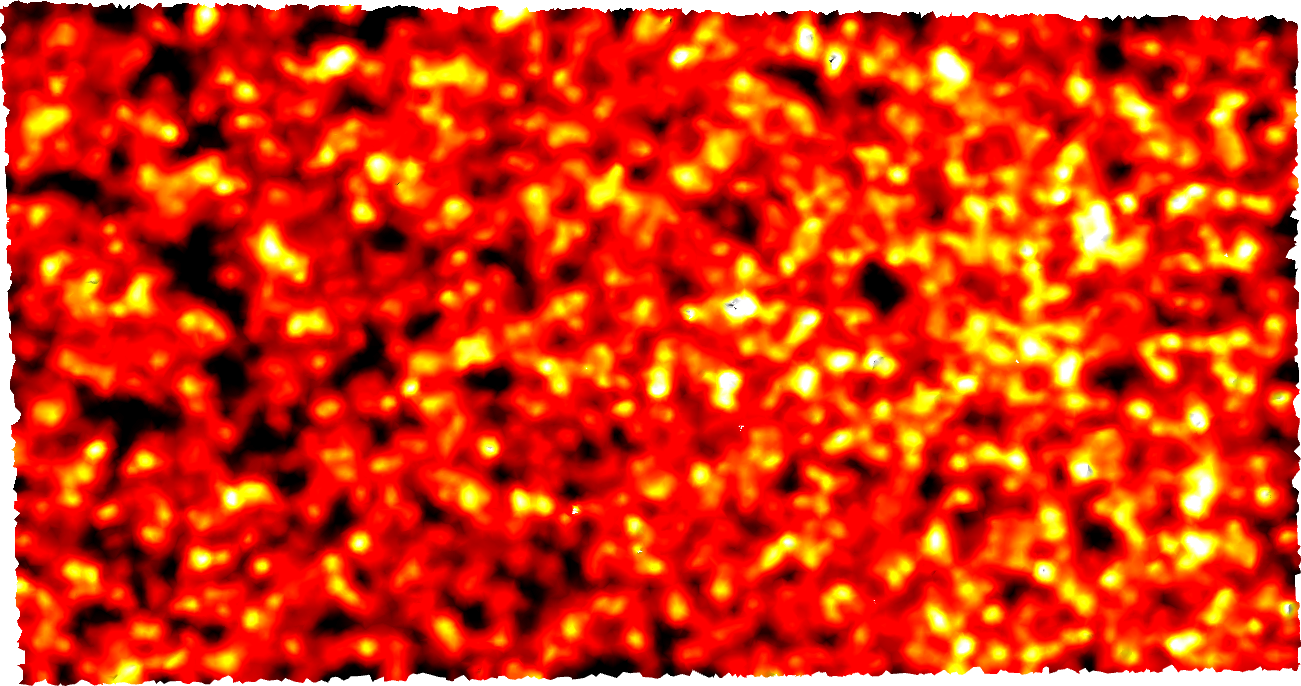
\includegraphics[width=\linewidth]
		{data/acquired_meshes/ILATO_1A_SM2066-HE5-60_070214_merged_GMO_r1_n4_v256_funcvals_1000iter.png}
		\caption{$c=1000$}\label{fig:ILATO.c}
	\end{subfigure}
	\begin{subfigure}[b]{0.49\linewidth}
		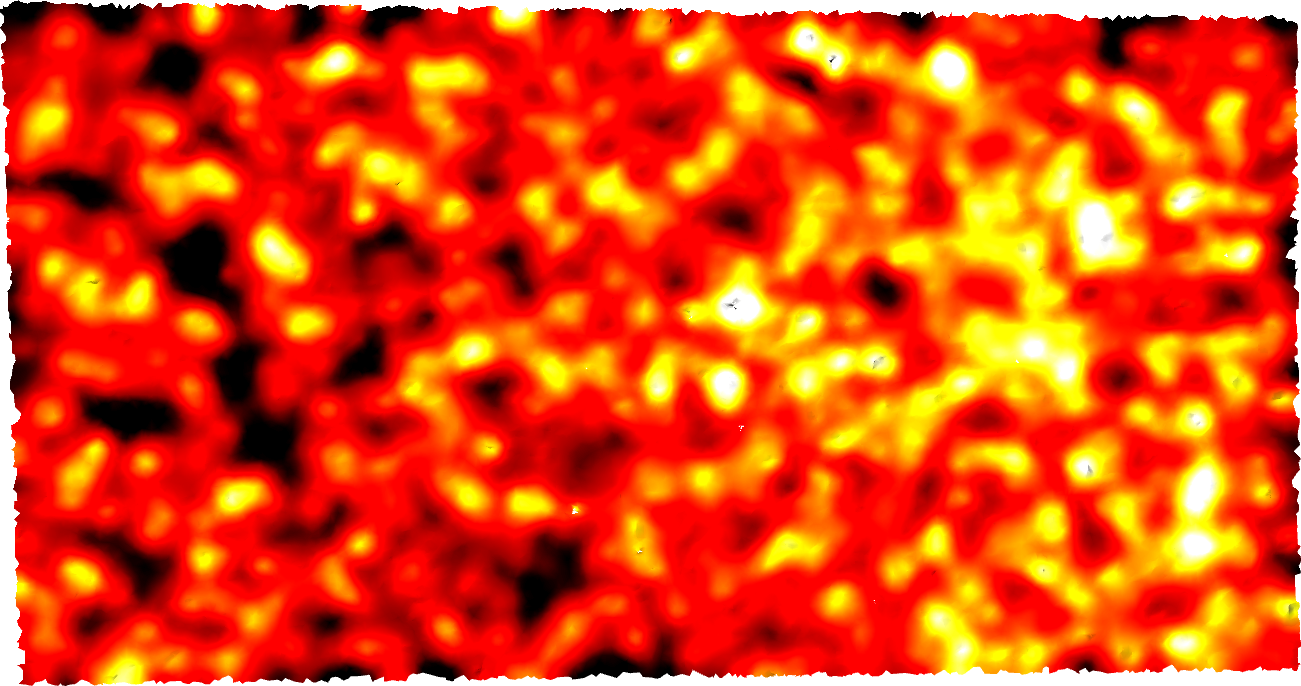
\includegraphics[width=\linewidth]
		{data/acquired_meshes/ILATO_1A_SM2066-HE5-60_070214_merged_GMO_r1_n4_v256_funcvals_3000iter.png}
		\caption{$c=3000$}\label{fig:ILATO.d}
	\end{subfigure}
	\caption[Four Views of the Flat Surface from ILATO]{Four views of a flat surface (a) in wireframe (b) colored by MSII function value before convolving the filter (c) colored by function value after convolving the filter 1,000 times (c) and after 3,000 times.}
	\label{fig:ILATO}
\end{figure}


As with the other acquired \tdd{}, the function values were computed by applying the MSII filter and use the same color ramp as the other models, however, because total variance over the entire model is very small, in the range of -0.018 and 0.018, practically representing the noise characteristic of the 3D-scanner and software used to generate the mesh, the range of function values are also compressed, so smoothing does not appear to occur as rapidly as seen in other experiments which is expected.

%
%
%
%
\subsection{The Stanford Bunny}
\label{ch6sATDDssSB}
The Stanford Bunny was range scanned in 1994 using a Cyberware 3030MS optical triangulation scanner. The ten separate scans were then zippered together~\cite[Turk94] to produce the \tdd{} which we obtained from The Stanford 3D Scanning Repository~\cite{StanfordBun}. This mesh is comprised of 35,947 points and 69,451 faces.

Figure~\ref{fig:bun} shows three views of the Stanford Bunny: in wireframe, colored by function values generated by applying \gls{tMSIIf}, before convolving \fors{t}, and colored by function value after convolving \fors{t} 100 times.
\begin{figure}[ht]
	\begin{subfigure}[b]{0.32\linewidth}
		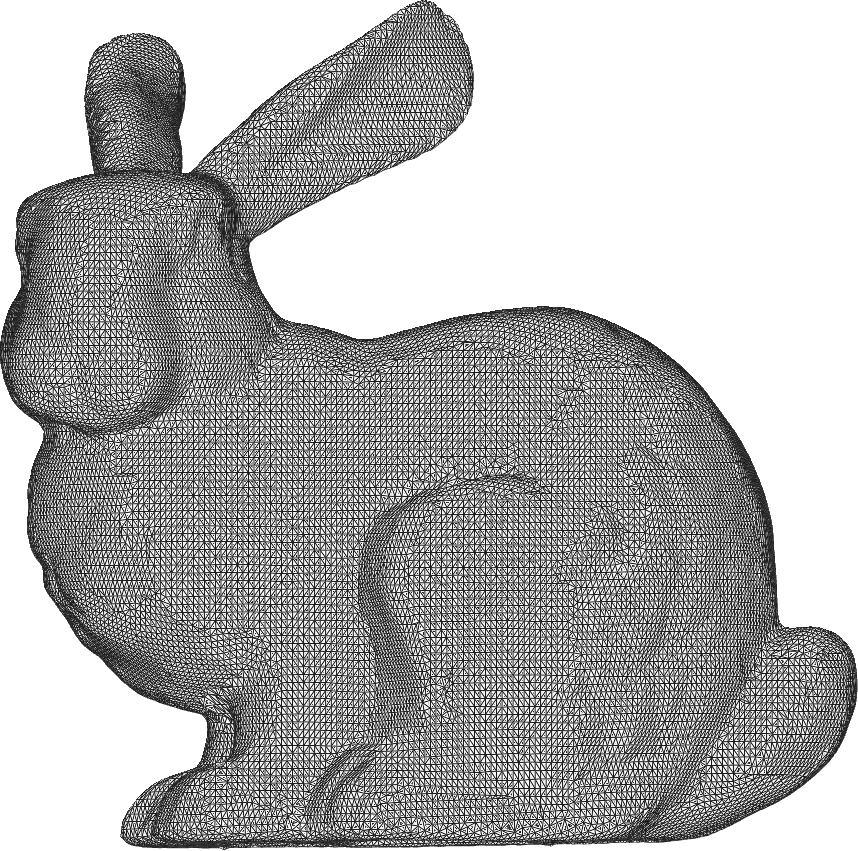
\includegraphics[width=\linewidth]
		{data/acquired_meshes/bun_zipper_edited_r1_n4_v256_wireframe.png}
		\caption{wireframe}\label{fig:bun.a}
	\end{subfigure}
	\begin{subfigure}[b]{0.32\linewidth}
		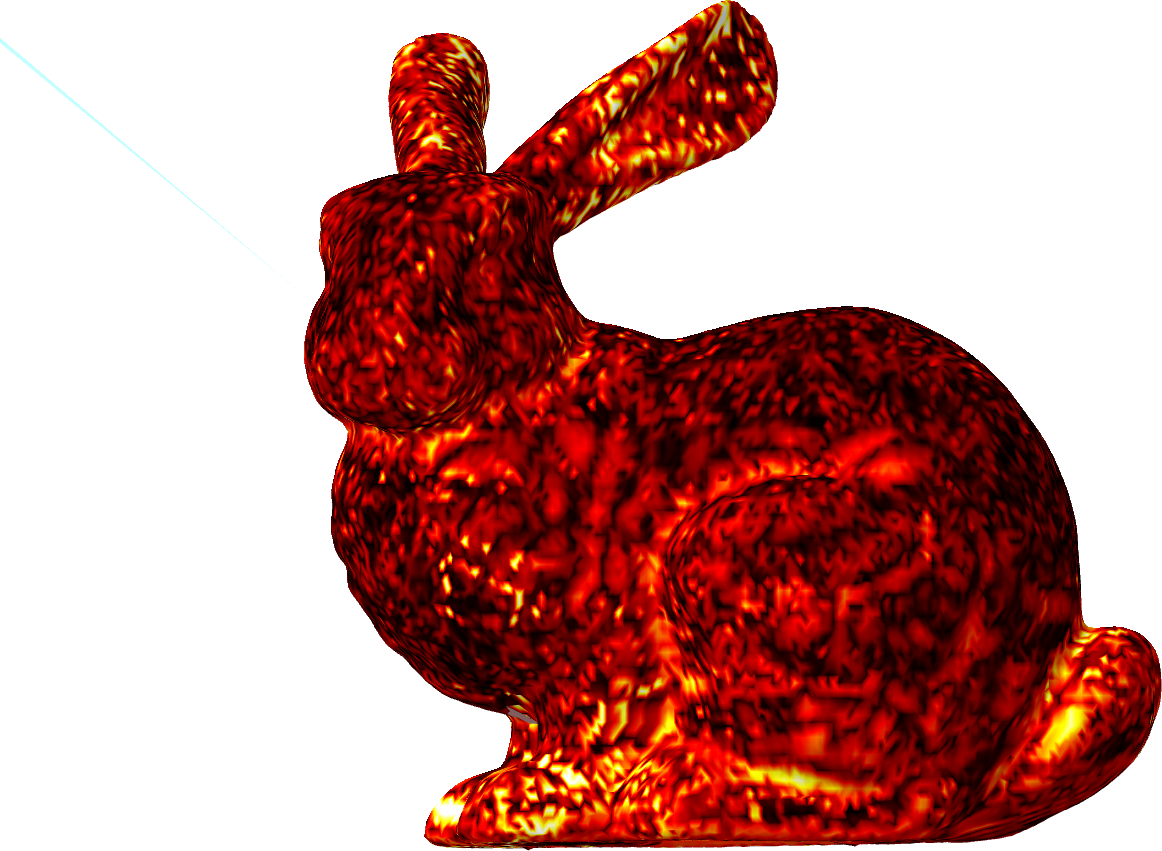
\includegraphics[width=\linewidth]
		{data/acquired_meshes/bun_zipper_edited_r1_n4_v256_funcvals_0iter.png}
		\caption{$c=0$}\label{fig:bun.b}
	\end{subfigure}
	\begin{subfigure}[b]{0.32\linewidth}
		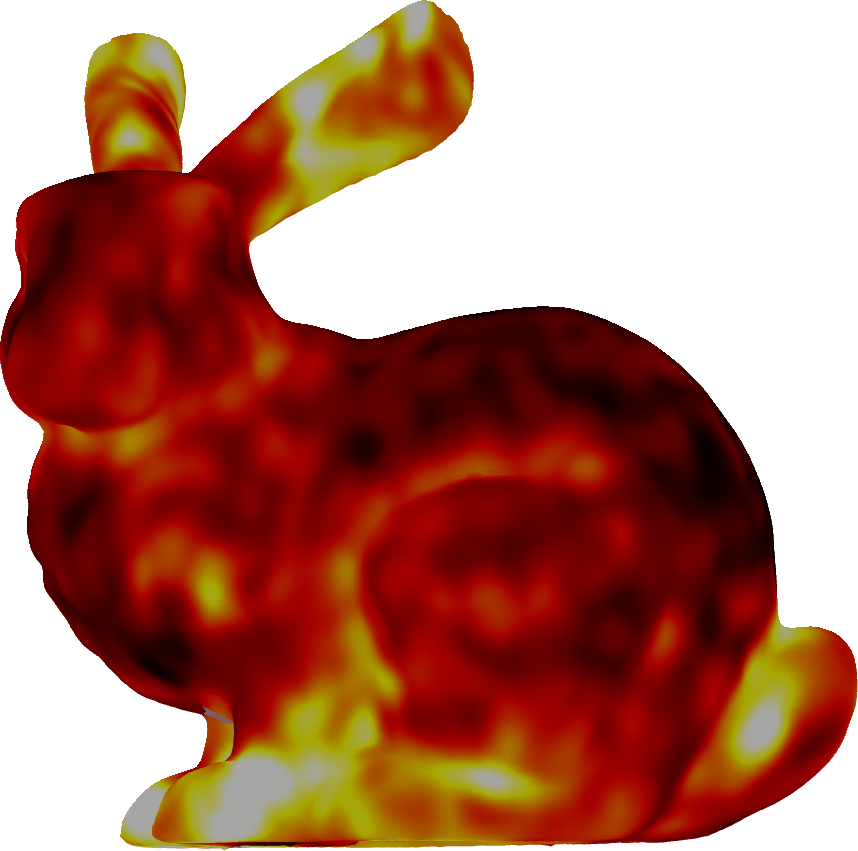
\includegraphics[width=\linewidth]
		{data/acquired_meshes/bun_zipper_edited_r1_n4_v256_funcvals_100iter.png}
		\caption{$c=100$}\label{fig:bun.c}
	\end{subfigure}
	\caption[Three Views of the Stanford Bunny]{Three views of the Stanford Bunny (a) in wireframe, (b) colored by \gls{tMSIIf} value before convolving the filter, and (c) colored by function value after convolving the filter 100 times.}
	\label{fig:bun}
\end{figure}


In this section, we presented three examples of acquired \tdd{} and experienced some of the difficulties inherent to processing and analyzing irregular triangle meshes. Without first cleaning the mesh, we experience error propagation with the university seal, and because of the relatively small variance in the function values of the flat surface, we experience a slow down in the effectiveness of the filter. In the next section we present and evaluate the results of the multitude of experiments conducted in order to establish the performance of the parallel variant of \Fors{t} algorithm.

%
%
%
%
%
%
\section{Convolving with a GPGPU}
\label{ch6sCWG}
In this section we present the collection of experiments performed with the goal of establishing the speedup and efficiency obtained when convolving \Fors{t} utilizing the \gls{SIMD} concurrency architecture provided by \glspl{GPGPU}. To that end, first the optimal sequential execution time, and the parallel compute time for the two variants of the \fors{t} algorithm are established, as described in Section~\ref{ch6sCWGssCT}, then the speedup obtained for each pair of experiments is analyzed in Section~\ref{ch6sCWGssS}, followed by an analysis of the efficiency of each pair of experiments in Section~\ref{ch6sCWGssE}. Finally concluding about the efficacy of our implementation of the parallel variant of \fors{t} algorithm.

%
%
%
%
\subsection{Compute Times}
\label{ch6sCWGssCT}
Before we are able to evaluate the \gls{speedup} and \gls{efficiency} of the parallel variant of \Fors{t}, as discussed in Section~\ref{ch2sPPssEAPA}, we must first obtain two essential timings: the optimal sequential execution time $\mathit{T_s}$, and the parallel compute time $\mathit{T_{\rho}}(\hat{n},\,\rho)$. In order to establish these values, we generated four versions each of the synthetic bisected square tessellation and the synthetic hexagonal tessellation, using the members of the set \{1, 10, 100, 1000\} as parameter $r$. Combined with the two acquired meshes, the university seal and the flat surface, that totaled ten meshes ranging in sizes from just nine points and eight faces, to $9\times 10^6$ points and $1.8\times 10^7$ faces.

Next, we designated two machines, a laptop M, and a desktop T, each with a CPU for serial computation as well as a GPU for parallel processing, in order to obtain comparisons across hardware of differing capabilities. T operates on a Intel(R) Core(TM) i7-8700 CPU @ 3.20GHz, while M operates on a Intel(R) Core(TM) i5-7300HQ CPU @ 2.50GHz. T has installed a NVIDIA Corporation GP104GL [Quadro P5000] GPU with 2,560 CUDA cores~\cite{quadro5k}, while M has installed a NVIDIA Corporation GP107M [GeForce GTX 1050 Ti Mobile] with 768 CUDA cores~\cite{geforce1050}.

Then, we systematically executed every combination\footnote{Of the 320  combinations of experiments, we were only able to record data for 309 different combinations because of the memory limitations of the laptop M. However, given the strong trends already established, it is uncertain that any additional data would influence the conclusions we draw about the reported experiments.} of hardware and mesh for eight increasing amounts of convolutions, \{1, 3, 10, 30, 100, 300, 1000, 3000\}, restarting the count for each experiment in order to ensure that the resulting time was genuine.

For the serial algorithm, the implementation existing in the GigaMesh\todoCitation{gigamesh} framework was used, for the parallel algorithm, a new implementation in CUDA extended C++\todoCitation{cuda in C++} was developed and used. Verification of final resulting scalar field of \wmfv{s} were conducted at the conclusion of each pair of experiments, and it was determined that zero difference between the output of the serial algorithm vs the parallel variant; even with the largest meshes for the most convolutions.

Figure~\ref{fig:computeTimesLP} shows the timing results of every recorded experiment. The graph is drawn extra tall to ensure that the grid remains square for an unbiased assessment of the correlations therein. Results from each combination of hardware and mesh are connected by lines.
%\todoResearch{add formula for timing (or at least ref to it) here.}
%\todoResearch{process time noise at very fast speeds}

\begin{figure}[ht]
\includegraphics[width=1.0\linewidth,height=1.0\textheight,keepaspectratio]
	{figures/computeTimesLinespoints.png}
	\caption[Compute Times per Experiment for increasing Convolution Counts]{Compute times per experiment for Increasing numbers of convolutions of \fors{t} onto acquired and synthetic \tdd{} of varying sizes. Combinations involving the smallest mesh sizes are colored red, and the largest mesh sizes in blue, with all others scaled in-between. The experiments involving acquired \tdd{} are specially marked with squares for the flat surface mesh, and circles for the university seal.

\vspace*{\baselineskip}
\scriptsize† The experiment codes used correspond to: the machine, T for the desktop or M for the laptop; the algorithm variant, P for parallel or S for serial; the mesh being processed, BS for bisected square, HT for hexagonal tessellation, US for university seal, and FS for the flat surface; and finally, the count of points comprising the mesh.}
	\label{fig:computeTimesLP}
\end{figure}

Notice how the compute times increase linearly with both mesh size and number of iterations. Timing is very predictable when the total compute time is at least greater than 0.1 seconds, but is much less predictable for faster periods. Fortunately, the deviations from the trends only occur for short total total timings, and do not appear to propagate per convolution for medium or long compute times, therefore they are unlikely to be noticed by the typical user.

Figure~\ref{fig:computeTimesS} plots the total compute times of each experiment as the area of a circle\footnote{The areas of the circles were to be scaled by the cube root of the actual size, so that the smallest circle is barely visible, and the largest remains within the border of the graph, and the general growth trend is still recognizable.}, given different hardware and algorithm configurations, for each combination of mesh size, measured in point counts, and number of convolutions of \fors{t}.

In general, one can see that for all experiments, the total compute times increase with the size of the mesh, as well as the number on convolutions, so that an increase in both results in an exponential increase in the compute time. Which is as expected given the complexity of the algorithm as discussed in Chapter~\ref{ch3}. One can also see the positive effect of the parallel processing, as the growth of the compute times is much slower for the parallel variant than for the serial.

\begin{figure}[ht]
	\includegraphics[width=\linewidth]{figures/computeTimesScatter.png}
	\caption[Compute Times Scatter Plot]{A plot of the total compute times of each experiment as the area of a circle, given different hardware configurations, for each combination of mesh size, measured in point counts, and the number of convolutions of \fors{t}. Blue circles indicate the serial variant computed with a \gls{CPU}, and a red circle indicating the parallel variant was computed on a \gls{GPGPU}.

\vspace*{\baselineskip}
\scriptsize† See Figure\ref{fig:computeTimesLP} for an explanation of the experiment codes.}
	\label{fig:computeTimesS}
\end{figure}

In this section, we endeavored to establish the optimal sequential execution time $\mathit{T_s}$, and the parallel compute time $\mathit{T_{\rho}}(\hat{n},\,\rho)$ given different hardware configurations and mesh sizes. In addition to the timing values, we also discovered a few trends characteristic of \fors{t}. In the next section, we will continue our evaluation by calculating the speedup and efficiency obtained by processing the parallel variant of the filter algorithm using \glspl{GPGPU}.

%
%
%
%
\subsection{Speedup}
\label{ch6sCWGssS}
Having now establish the optimal sequential execution time $\mathit{T_s}$, and the parallel compute time $\mathit{T_{\rho}}(\hat{n},\,\rho)$ of \Fors{t}, we can now continue our evaluation by calculating, as discussed in detail in Section~\ref{ch2sPPssEAPA}, the \gls{speedup} obtained by convolving the filter over different sized meshes in parallel using \glspl{GPGPU}.

Figure~\ref{fig:speedup} is a plot of the \gls{speedup} obtained by convolving the parallel variant of \fors{t} over meshes of different sizes for increasing number of convolutions, using either the \gls{GPGPU} of the laptop M with 768 \gls{CUDA} cores or the \gls{GPGPU} of desktop T with 2,560 \gls{CUDA} cores.

\begin{figure}[ht]
	\includegraphics[width=\linewidth]{figures/speedup.png}
	\caption[Speedup]{A graph of the \gls{speedup} obtained by convolving the parallel variant of \Fors{t} over meshes of different sizes. Lines in blue, increasing in saturation with the size of the mesh, are experiments run using the \gls{GPGPU} of laptop M with 768 \gls{CUDA} cores. Lines in red, increasing in saturation with the size of the mesh, are experiments run using the \gls{GPGPU}  of desktop T with 2,560 \gls{CUDA} cores. The experiments involving acquired \tdd{} are specially marked with squares for the flat surface mesh, and circles for the university seal.

\vspace*{\baselineskip}
\scriptsize† See Figure\ref{fig:computeTimesLP} for an explanation of the experiment codes.}
	\label{fig:speedup}
\end{figure}

One general trend which emerges is that for both hardware configurations, more speedup can be gained when convolving the filter on meshes of larger sizes. This can be explained by the increase in the \gls{degreeOfPar} which comes with meshes with large counts of points, and is related to \gls{Amdahl}, as discussed in Section~\ref{ch2sPPssEAPA}.

Also, in general but especially for larger meshes, convolving the filter using the \gls{GPGPU} of the desktop T garners high speedup than the equivalent experiments using the laptop M hardware configuration. This is expected, because as the \gls{degreeOfPar} increases with mesh size, the higher number of \gls{CUDA} cores available to T allow it to processes more computations in parallel than M; although never reaching the ratio of 2,560 to 768 that one might expect, as discussed in more detail in the next section, Section~\ref{ch6sCWGssE}.

Another trend is that for most configurations, speedup increases with increasing number of convolutions, seeming to converge to a certain number. More research must be done in order to determine why this may be, but it is possible that it is related to low-level memory optimization by the operating system.

A third trend, which may not be easily seen in the graph is that for the smallest-sized meshes, the speedup is less than one, indicating a slow down in compute time. In fact, the minimum speedup obtained in our experimentation was with the synthetic bisected square tesselation generated with parameter $r=1$, consisting of only nine points, which has a speedup of $\approx$0.35 when convolving with the parallel filter on desktop T's \gls{GPGPU} 3,000 times. That equates with performing three times as slow as the equivalent serial experiment, and is likely due to the overhead incurred by the necessary usage of locking mechanisms and explicit thread synchronization in the parallel variant of the algorithm.

Fortunately, the speedup obtained by convolving the parallel variant of \fors{t} using GPGPUs, is overall quite high. The maximum speedup obtained by any experiment was $\approx$204.43, which equates to the parallel variant performing 200 times as quick than the serial algorithm. This speedup was obtained when convolving the parallel variant of the filter, for 3,000 convolutions, on the synthetic quadrisected square tesselation generated with parameter $r=1000$, consisting of more than four million points, using desktop T's \gls{GPGPU}.

Also notable, the acquired \tdd{} enjoyed appreciable speedup, though considerably less than the synthetic meshes of equivalent sizes. The flat surface mesh obtained the maximum speedups of $\approx$60.25 with the laptop M's \gls{GPGPU} and $\approx$102.74 when using desktop T's \gls{GPGPU}. While the bisected square tessellation generated with parameter $r=100$ peaked at $\approx$103.67 with M and $\approx$154.80 with T, despite being smaller. Likewise, the university seal obtained the maximum speedups of$\approx$60.08 with the laptop M's \gls{GPGPU} and $\approx$113.10 when using desktop T's \gls{GPGPU}, while the similarly-sized quadrisected square tessellation peaked at $\approx$115.62 with M and $\approx$204.43 with T. It is unclear what caused these dependencies, but we speculate that it may be due to wider the variance in neighborhood size and function values present in \tdd{}, when compared to synthetic \tdd{}.

%
%
%
%
\subsection{Efficiency}
\label{ch6sCWGssE}
In this section we evaluate the other important metric for analyzing the performance of a parallel algorithm, \gls{efficiency}, as discussed in detail in Section~\ref{ch2sPPssEAPA}. Having establish the optimal sequential execution time $\mathit{T_s}$, and the parallel compute time $\mathit{T_{\rho}}(\hat{n},\,\rho)$ of \Fors{t}, \gls{efficiency} is calculated as \gls{speedup}, divided by the number of processors used to obtain it.

Figure~\ref{fig:efficiency} is a plot of the \gls{efficiency} obtained by convolving the parallel variant of \fors{t} over meshes of different sizes for increasing number of convolutions, using either the \gls{GPGPU} of the laptop M with 768 \gls{CUDA} cores or the \gls{GPGPU} of desktop T with 2,560 \gls{CUDA} cores.

\begin{figure}[ht]
	\includegraphics[width=\linewidth]{figures/efficiency.png}
	\caption[Efficiency]{A graph of the \gls{efficiency} obtained by convolving the parallel variant of \fors{t} over meshes of different sizes. Lines in blue, increasing in saturation with the size of the mesh, are experiments run using the \gls{GPGPU} of laptop M with 768 \gls{CUDA} cores. Lines in red, increasing in saturation with the size of the mesh, are experiments run using the \gls{GPGPU} of desktop T with 2,560 \gls{CUDA} cores. The experiments involving acquired \tdd{} are specially marked with squares for the flat surface mesh, and circles for the university seal.

\vspace*{\baselineskip}
\scriptsize† See Figure\ref{fig:computeTimesLP} for an explanation of the experiment codes.}
	\label{fig:efficiency}
\end{figure}

The most noticeable trend in Figure\ref{fig:efficiency} is that experiments ran using the laptop M hardware configuration obtain higher efficiency that the equivalent experiments ran using the desktop T hardware configuration. This trend is attributable to the design of the parallel algorithm, which is unable to scale effectively and utilize the increase in processor count provided by the \gls{GPGPU} of T.

Secondly, the efficiency obtained when convolving the filter on acquired \tdd{} is approximately only half of the efficiency obtained when convolving the filter on similarly sized synthetic meshes. This is a direct consequence of causes behind the slower speedup for \tdd{} as calculated in the previous section.

The maximum efficiency recorded is $\approx$0.151, and was obtained when convolving \fors{t} 3,000 times on the bisected square tessellation with four million points. This equates to only 15\% of total processor effort effectively contributing to the final values.

The minimum efficiency recorded is $\approx$0.000136, and similar to the minimum speedup, was obtained when convolving \fors{t} 3,000 times on the bisected square tessellation with only nine points. This equates to only .01\% of total processor effort effectively contributing to the final values.

%
%
%
%
%
%
\clearpage
\section{Summary}
The goal of our experimentation was two-fold, analyzing the filter response on various kinds of \tdd{} as well as evaluating the performance of the parallel variant of \fors{t} algorithm. Therefore, we began in Section~\ref{ch6sSTDD} by analyzing the filter response when convolving the filter of over four different configurations of synthetic \tdd{}, each with the \gls{ddf} applied as a scalar field.

Some anisotropic behavior was exhibited by \fors{t} response traveling faster along the connections of more distant adjacent points, while isotropic behavior was exhibited when the overall variance in the length of edges was reduced. The filter response also appeared to slow down when convolved over irregular meshes, more similar to acquired \tdd{}.

Next, in Section~\ref{ch6sATDD} we analyzed the filter response when convolving the filter of over three different examples of acquired \tdd{} where an error in computation was seen propagating across the image with each subsequent convolution, as well as the efficacy of the response of the filter diminishing when convolving the filter over a scalar field with very low variance.

Then in Section~\ref{ch6sCWG}, we established the compute times for a multitude of pairs of experiments, involving both the serial sand parallel algorithm, both acquired and synthetic \tdd{}, and four different configurations of hardware.

In the next chapter, we will combine everything that we have discovered through our research, and make conclusions about \Fors{t} in general, and its parallel variant utilizing \glspl{GPGPU}.
